\documentclass[12pt]{article}
\usepackage{amssymb,amsmath,natbib,graphicx,amsthm,
  setspace,sectsty,anysize,times,dsfont,enumerate}

\usepackage[svgnames]{xcolor}

\usepackage{lscape,arydshln,relsize,rotating,multirow}
\usepackage{caption}
\captionsetup{%
  font=small,
  labelfont=normalfont,
  singlelinecheck=false,
  justification=justified
}
\usepackage{algorithm,algorithmic}

\graphicspath{{/Users/mtaddy/project/gamma_lasso/graphs/}}
\newtheorem{prop}{\sc Proposition}[section]
\newtheorem{theorem}{\sc Theorem}[section]
\newtheorem{definition}{\sc Definition}[section]
\newtheorem{lemma}{\sc Lemma}[section]
\newtheorem{corollary}{\sc Corollary}[section]

\marginsize{1.1in}{.9in}{.3in}{1.4in}

\newcommand{\nb}{\color{blue}}
\newcommand{\dbl}{\setstretch{1.5}}
\newcommand{\sgl}{\setstretch{1.2}}

\newcommand{\bs}[1]{\boldsymbol{#1}}
\newcommand{\mc}[1]{\mathcal{#1}}
\newcommand{\mr}[1]{\mathrm{#1}}
\newcommand{\bm}[1]{\mathbf{#1}}
\newcommand{\ds}[1]{\mathds{#1}}
\newcommand{\indep}{\perp\!\!\!\perp}
\DeclareMathOperator*{\argmin}{argmin}
\newcommand{\norm}[1]{|\!|#1|\!|_{1}}
\newcommand{\code}[1]{{\smaller\sf#1}}
\newcommand{\e}[1]{{\footnotesize$\times10$}{$^{#1}$}}

\usepackage[bottom,hang,flushmargin]{footmisc}

\pdfminorversion=4
\begin{document}

\sgl 

\pagestyle{empty}

~
\vskip 3cm

\noindent {\LARGE \bf One-step estimator paths for concave regularization} 

\vskip 1cm

\noindent{\Large Matt Taddy}

{\large
\vskip .5cm \noindent
{The  University of Chicago Booth School of Business}\\
\texttt{faculty.chicagobooth.edu/matt.taddy}}



\vskip 2cm

{\noindent This article explores some practical and computational issues
related to the application of sparse diminishing-bias regularized regression:
techniques which mimic estimation under coefficient penalty functions spanning
the range of concavity between $L_0$ and $L_1$ norms. In Big data
applications, where exact solvers are too computationally expensive, such
techniques reduce largely to $L_1$ regularization with data-dependent weights.
We present novel results on the distance between weighted-$L_1$ penalized
minimization and $L_0$ minimization, giving some intuition on the amount of
information compression that is possible.  We then propose a simple new
algorithm framework -- the path of one-step estimators (POSE) -- which does
$L_1$ penalized regression estimation on a grid of decreasing penalties, but
adapts coefficient-specific weights to decrease as a function of the 
coefficient estimated in the previous path step.  POSE provides the benefits of
diminishing-bias, but at a computational cost close or equal to that of the
standard lasso.  One specific implementation of POSE, the `gamma lasso', is
motivated from Bayesian foundations and we work through the details necessary
for its application.  The methods and issues discussed are illustrated through
use of the gamma lasso in extensive linear regression simulations and in
application of logistic regression to evaluating the performance of hockey
players.}
 

\newpage
\dbl

\pagestyle{plain}
\vskip 1cm
\section{Introduction}
\label{intro}

For regression in high-dimensions, it is useful to regularize estimation
through a penalty on coefficient size.   $L_1$  regularization \citep[i.e.,
the lasso of][]{tibshirani_regression_1996} is especially popular, with costs
that are non-differentiable at their minima and can lead to  coefficient
solutions of exactly zero.  A related approach is that of concave penalized
regularization (e.g. SCAD from \citealt{fan_variable_2001} or MCP from
\citealt{zhang_nearly_2010}) with cost functions that are also spiked at zero
but flatten for large values (as opposed to the constant increase of an $L_1$
norm).  This yields sparse solutions where the large non-zero values are estimated
with little bias. The combination of  \textit{sparsity} and \textit{diminishing-bias} 
 is appealing in many settings, and a large literature on concave
penalized estimation has developed over the past 15 years.  For example, many
authors (e.g., from \citealt{fan_variable_2001} and
\citealt{fan_nonconcave_2004})  have contributed work on their \textit{oracle
properties}, a class of results showing conditions under which coefficient
estimates through concave penalization, or in related schemes, will be the same
as if you knew the sparse `truth'.

Unfortunately,  exact solvers for concave penalized estimation  all require
significantly more compute time than a standard lasso.  As we review in
Section \ref{rp}.1,  recent literature recommends the use of approximate
solvers.  Certainly, this is necessary for data of the size we encounter in
analysis of, say, internet commerce.  These approximations  take the form of
iteratively-weighted-$L_1$ regularization, where the coefficient-specific
weights are based upon pre-estimates of the coefficients taken from previous
iterations of the approximate solver.  One theme of this literature
\citep[e.g.,][]{zou_one-step_2008,fan_strong_2014} 
holds that even a single step of weighted-$L_1$ regularization is enough to
get solutions that are close to optimal, so long as the pre-estimates
are \textit{good enough} starting points. The crux of success with such one-step
estimation (OSE) is  finding starts that are, indeed, good enough.

This article presents a computational strategy for obtaining a {\it path} of
 one-step estimates under concave penalization.  The generic POSE -- path of
 one-step estimators -- algorithm simply uses each solution along a
 regularization path as the basis for weights at the next path iteration. In
 this way, we are able to achieve  near-lasso speeds while obtaining a path of
 sparse diminishing-bias estimators.  Our implementation and illustrations
 apply POSE using the log penalty
 \citep[e.g.][]{candes_enhancing_2008}, and we refer to this as the `gamma
 lasso'  for its interpretation as the posterior mode under a hierarchical Bayesian model.
However, we make no claims for theoretical superiority for one target penalty over another.  Rather, we treat one-step weighted-$L_1$ estimators at face-value and address practical issues in computation for such schemes:
\begin{itemize}
\item minimizing the cost of computing good pre-estimates,
\item moving quickly along a path of candidate estimators, and
\item having tools available for selection amongst these candidates.
\end{itemize}
All three issues are related to each other, and we will illustrate their interdependency.

Section \ref{rp} is a survey of sparse diminishing-bias
regularization: we
review the connection between concave and weighted-$L_1$ penalties in
\ref{rp}.1, and present novel results on the distance between weighted-$L_1$
 and $L_0$ minimization in \ref{rp}.2. The POSE algorithm is introduced in
Section \ref{pose}, with our  gamma lasso specification in \ref{pose}.1 and its motivation from Bayesian foundations in \ref{pose}.2.  Section \ref{sss}  covers
implementation issues key to any path-based strategy:  speed and stability
in \ref{sss}.1, and model selection  in \ref{sss}.2.  Finally, Section
\ref{eg} presents two empirical studies:
a  simulation experiment in \ref{eg}.1, and in \ref{eg}.2 we investigate the data analysis question: given all goals in the past decade of NHL hockey, what can we say about individual player contributions? 

Throughout,
we focus on practice and computation.  For example, the theory of Section
\ref{rp}.3 and the experiment in Section \ref{eg}.1 take $L_0$
minimization as the oracle comparator. We are agnostic about existence of
any sparse `truth' and promote these techniques from an
 information-compression perspective. And Section \ref{sss} emphasizes
quick selection amongst a range of penalty sizes, as required
by any practitioner who is unwilling to rely upon theoretically
optimal specification when analyzing real data. The goal is to help nudge
sparse diminishing-bias regularization into the Big Data
mainstream.\footnote{To this end, we also provide polished and well-documented
software in the
\texttt{gamlr} package for R.}


\section{Sparse regularization paths and diminishing bias}
\label{rp}

Denote $n$ response observations as $\bm{y} = [y_1,\ldots,y_n]'$ and the associated matrix of $p$ covariates as $\bm{X} =
[\bm{x}_1 \cdots \bm{x}_n]'$, with rows $\bm{x}_i = [x_{i1},\ldots,x_{ip}]'$ and columns $\bs{x}_j = [x_{1j},\ldots,x_{nj}]'$.\footnote{Since the size of penalized $\beta_j$ depends upon the units of $x_{ij}$,  it is common to scale
the coefficient by $\mr{sd}(\bs{x}_j)$, the standard deviation of the $j^{th}$ column
of $\bm{X}$; this is achieved if $x_{ij}$ is replaced by $x_{ij}/\mr{sd}(\bs{x}_j)$
throughout.} Write $\eta_{i} =
\alpha+\bm{x}_i'\bs{\beta}$ as the linear equation for observation $i$, and
denote with $l(\alpha, \bs{\beta}) = l(\bs{\eta})$  an unregularized
objective  proportional to the negative log likelihood.  For example, in Gaussian (linear)
regression, $l(\bs{\eta})$ is the sum-of-
squares $0.5\sum_i \left(y_i - \eta_i\right)^2$ and in binomial (logistic)
regression,  $l(\bs{\eta}) = -\sum_i \left[\eta_iy_i -
\log(1+e^{\eta_i})\right]$ for $y_i \in [0,1]$.  
A penalized estimator is then the solution to
\begin{equation} \label{pendev}
{\min}\left\{~l(\alpha,{\bs{\beta}}) + n\lambda \sum_{j=1}^p c_j(|\beta_j|)~\right\},
\end{equation}
where $\lambda>0$ controls overall penalty magnitude and are $c_j()$ are coefficient cost functions.
 
\begin{figure}[t]
\vspace{-.5cm}
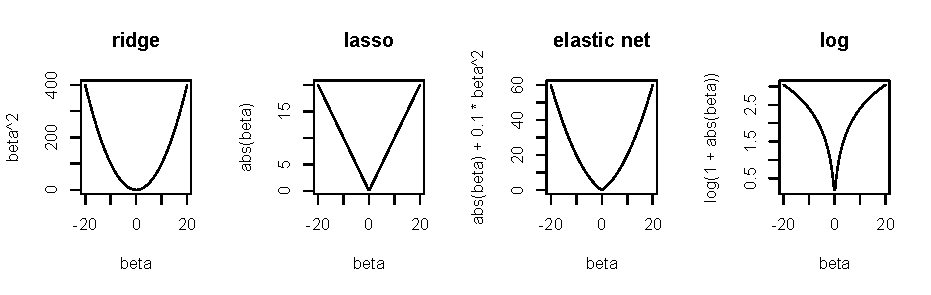
\includegraphics[width=6.25in]{penalties}
\vskip -.5cm
\caption{\label{costs} 
From left to right, 
$L_2$ costs \citep[ridge,][]{hoerl_ridge_1970}, $L_1$ \citep[lasso,][]{tibshirani_regression_1996}, the `elastic net' mixture of $L_1$ and $L_2$ \citep{zou_regularization_2005}, and the log penalty \citep{candes_enhancing_2008}.
}
\end{figure}

A few common cost functions are shown in Figure \ref{costs}.  Those that have
a non-differentiable spike at zero (all but ridge) lead to sparse estimators,
with some coefficients set to exactly zero.   The curvature of the penalty
away from zero dictates then the weight of shrinkage imposed on the nonzero
coefficients:  $L_2$ costs increase with coefficient size,  lasso's $L_1$
penalty has zero curvature and imposes constant shrinkage, and as curvature
goes towards $-\infty$ one approaches the $L_0$ penalty of subset selection.
In this article we are primarily interested in {\it concave} cost functions,
like the log penalty, which span the range between $L_1$ and $L_0$ penalties.

The penalty size, $\lambda$, acts as a {\it squelch}: it suppresses noise to
focus on the true input signal. Large $\lambda$ lead to very simple 
model estimates, while as $\lambda \rightarrow 0$ we approach maximum
likelihood estimation (MLE). Since you don't know optimal $\lambda$,
practical application of penalized estimation requires a {\it regularization
path}: a $p \times T$ field of $\bs{\hat\beta}$ estimates obtained while
moving from high to low penalization along $\lambda^1 > \lambda^2 \ldots >
\lambda^T$ \citep[e.g., LARS in][is a well known example]{efron_least_2004}.
These paths begin at $\lambda^1$ set to infimum $\lambda$ such that
(\ref{pendev}) is minimized at $\bs{\hat\beta} = \bm{0}$ (see Appendix
\ref{models}), and proceed down to some pre-specified $\lambda^T$ (e.g., $\lambda^T=
0.01\lambda^1$).

\subsection{Concave penalization}


\begin{figure}[t]
\vskip -.25cm
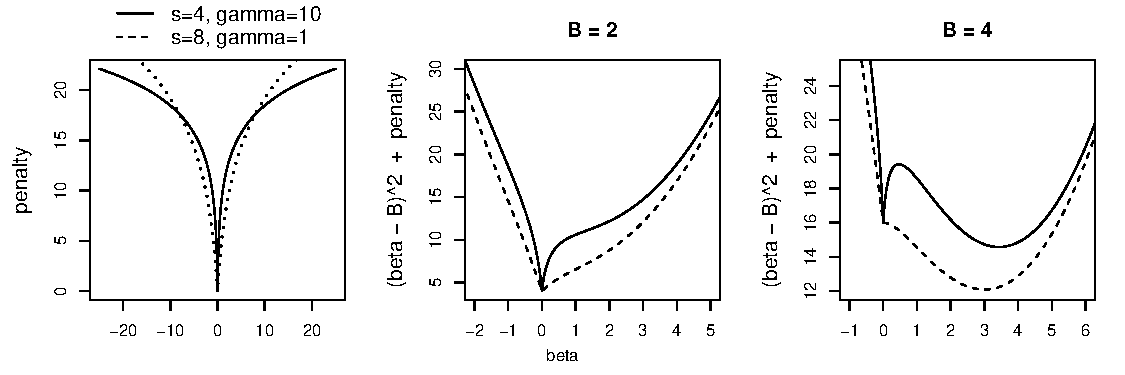
\includegraphics[width=6.4in]{solution}
\caption{\label{solution} Log penalties $c(\beta) = s\log(1 + \gamma|\beta|)$ 
and penalized objectives $(\beta-B)^2 + c(\beta)$.}
\end{figure}


Concave penalties such as the log penalty, which have a gradient that is
decreasing with absolute coefficient size,  yield the `diminishing-bias'
property discussed in the introduction. It is {\it the} reason why one would
use concave penalization instead of $L_1$ or convex alternatives.
Unfortunately, such penalties can overwhelm the convex likelihood and produce a 
concave minimization objective; see Figure \ref{solution} for illustration.


This concavity makes computation difficult.  For example,  one run of SCAD via
the \texttt{ncvreg} R package \citep{breheny_coordinate_2011} for the
simulation in Section \ref{eg}.1 requires around 10 minutes, compared to 1-2
seconds for the lasso.  The slowness is due to the difficulty of concave
minimization: finding global, or even good local, minima is an extremely tough
task.  The most efficient exact solver that we've found is the
\texttt{sparsenet} of \citet{mazumder_sparsenet_2011}, also implemented in R,
which first fits a lasso path under decreasing $L_1$ penalty magnitude and,
for each segment on this path, adapts coefficient estimates along a second
path of increasing penalty concavity. While far more efficient than previous
alternatives, \texttt{sparsenet}  relies upon solution over a large set of
penalty specifications\footnote{POSE shares with
\texttt{sparsenet} the idea of moving along a path of closely related
specifications, but does not require a grid in both  cost size and concavity.
Intuitively,  POSE runs  a path diagonally through this grid.}  
 and its compute cost remains much higher than for lasso
(e.g., 15-20 seconds in our simulation).

A relatively fast class of solvers for concave penalized estimators uses
local linear approximation \cite[LLA; e.g.,][]{candes_enhancing_2008}. LLA
replaces the concave cost function $c_j$  with its tangent at the current
estimate, $c_j'(\hat\beta_j)\beta_j$.  The objective is then just a weighted
$L_1$ penalized loss (solvable, say, as in Appendix \ref{implement}), and one
iterates between updating $c'(\hat\beta)$ and solving the implied $L_1$
penalized minimization problem.  \citet{zou_one-step_2008} present numerical
and theoretical evidence that  LLA does well in practice. Importantly, they
show that LLA does well even (or especially) if you {\it stop it after one
iteration}. This is an example of one-step estimation (OSE), a 
technique inspired by \cite{bickel_one-step_1975} that amounts to taking as
your estimator the first step of an iterative approximation to some objective.
Such early-stopping can be as good  as the full-step solution
{\it if} the initial estimates are good enough. 

OSE and similar ideas have had a resurgence in the concave penalization
literature recently, motivated by the need for faster estimation algorithms.
\cite{fan_strong_2014} consider early-stopping of LLA for folded concave
penalization  and show that, under strong sparsity assumptions about true
$\bs{\beta}$ and given appropriate initial values, OSE LLA is with high
probability an oracle estimator.   Zhang (2010,2013)
\nocite{zhang_analysis_2010,zhang_multi-stage_2013} investigates  
`convex relaxation' iterations, where estimates under convex regularization
 are the basis for weights in a subsequent penalized objective.  He shows that
 just one or two steps here is sufficient for obtaining oracle support
 recovery properties under much weaker conditions than required by a standard
 lasso.  \cite{wang_calibrating_2013} propose a two step algorithm that feeds
 lasso coefficients into a linear approximation to folded concave
 penalization.  These OSE methods are all closely related to  the adaptive lasso
\citep[AL;][]{zou_adaptive_2006}, which does weighted-$L_1$ minimization under
weights $\omega_j = 1/|\hat\beta^0_j|$, where $\hat\beta^0_j$ is an initial
guess at the coefficient value.  The original AL paper advocates using MLE
estimates for initial values, while
\cite{huang_adaptive_2008} suggest using marginal regression coefficients
$\hat\beta^0_j = \mr{cor}(\bm{x}_j,\bm{y})$.\footnote{We include marginal AL in our study
of Section \ref{eg}.1.}

OSE LLA, or a two-step estimator starting from
$\bs{\hat\beta}=0$ as suggested in \cite{fan_strong_2014} and
\cite{wang_calibrating_2013}, or any version of the adaptive lasso, are {\it all just weighted-$L_1$
minimization}. These methods differ only in how the
weights are constructed.  Regardless of which you prefer, weighted-$L_1$
penalties are likely to play a central role in diminishing-bias penalization
whenever the dataset is too large for use of exact concave penalty solvers.


\subsection{Comparison between weighted-$L_1$ and $L_0$ penalized estimation}


Sparse estimation will be useful for (and often used in) settings where the
true data generating process is non-sparse. This can be motivated from an
information compression  perspective -- e.g., in Big data settings such as
\cite{taddy_distributed_2013}, where many estimates need to be quickly
communicated across multiple machines -- or from a simple desire to minimize
complexity and focus decision making.    We are thus interested in $L_1$
penalization with data-dependent weights as a way to obtain fits that are as
sparse as possible without compromising predictive ability.  

Our oracle benchmark is estimation under $L_0$ costs, $c_j(\beta_j) =
\ds{1}_{\{\beta_j\neq0\}}$, for which global solution is practically
impossible. We present finite sample bounds on the
distance  between  $L_0$  and weighted
$L_1$ penalized estimation.  This comparison yields simple relationships that
make no assumptions about the underlying data model. Moreover, when we do make
standard assumptions about the data generating process, we are able to
quantify distance between weighted-$L_1$ estimates and a theoretically optimal
$L_0$ penalized estimator.


\subsubsection{Sparse Approximation for Prediction}

 For any support subset $S \subset \{1\ldots p\}$ with cardinality $|S|=s$ and
complement $S^c = \{1\ldots p\}\setminus S$, denote vectors restricted to $S$
as $\bm{\beta}_S = [\beta_j:j\in S]'$, matrices as $\bm{X}_S$, etc.  Use
$\bs{\beta}^S$ to denote the coefficients for ordinary
least-squares (OLS) restricted to $S$: that is, $\bs{\beta}^S_S =
(\bm{X}_S'\bm{X}_S)^{-1}\bm{X}_S'\bm{y}$ and $\beta^{S}_j = 0~\forall~j\notin
S$.  Moreover, $\bm{e}^S = \bm{y}-\bm{X}\bs{\beta}^S =
(\bm{I}-\bm{H}^S)\bm{y}$ are residuals and $\bm{H}^S =
\bm{X}_S(\bm{X}_S'\bm{X}_S)^{-1}\bm{X}_S'$ the hat (projection) matrix from OLS restricted to $S$.  We suppress intercepts throughout, and use $|\cdot|$ and $\|\cdot\|$ applied to vectors as the $L_1$ and $L_2$ norms, respectively.

We'll use the following simple result for stagewise regression -- iterative fitting of new covariates to the residuals of an existing linear model (as in, e.g., \citealt{goldberger_stepwise_1961}). 
\begin{lemma}\label{SSElemma}
Say $\mr{MSE}_S = \|\bm{X}\bs{\beta}^S-\bm{y}\|^2/n$ and 
$\mr{cov}(\bs{x}_j,\bm{e}^S) = \bs{x}_j'(\bm{y}-\bm{X}\bs{\beta}^S)/n$ are sample variance and covariances.  Then for any $j \in 1\ldots p$, 
\[
\mr{cov}^2(\bs{x}_j,\bm{e}^S) \leq \mr{MSE}_S - \mr{MSE}_{S\cup j}
\]
\end{lemma}
\begin{proof}
From the well-known property on the correlation coefficient ($R^2$) for linear models,   
in-sample correlation and variances are such that
\[
\frac{\mr{cov}^2(\bs{x}_j,\bm{e}^S)}{\mr{var}(\bs{x}_j)\mr{var}(\bm{e}^S)} = 1 - \frac{\mr{var}(\bm{e}^S-\tilde\beta_j\bs{x}_j)}{\mr{var}(\bm{e}^S)}
\]
where $\tilde\beta_j = \bs{x}_j'\bm{e}^S/(\bs{x}_j'\bs{x}_j)$ is the stagewise coefficient estimate.  Since $\mr{var}(\bs{x}_j)=1$, multiplying everything by $\mr{var}(\bm{e}^S)$ yields $\mr{cov}^2(\bs{x}_j,\bm{e}^S) =
\mr{var}(\bm{e}^S) - \mr{var}(\bm{e}^S-\tilde\beta_j\bs{x}_j)
\leq \mr{var}(\bm{e}^S) - \mr{var}(\bm{e}^{S\cup j})$.
The last inequality holds because $\bm{e}^{S\cup j}$, residuals from OLS on $\bm{X}_{S\cup j}$, have the smallest-possible sum of squares for that set of covariates.  With $\mr{var}(\bm{e}^S) = \mr{MSE}_S$, etc, we are done.
\end{proof}

In addition, we need to define {\it restricted eigenvalues} (RE) on the gram matrix $\bm{X}'\bm{X}/n$.  
\begin{definition}\label{redef}
The restricted eigenvalue is
$
\phi^2(L,S) = \min_{\{\bm{v}: \bm{v}\neq \bm{0},~|\bm{v}_{S^c}| \leq L\sqrt{s}\|\bm{v}_S\|\}}\frac{\|\bm{X}\bm{v}\|^2}{n\|\bm{v}\|^2}$.
\end{definition}
\noindent The specific RE in Definition (\ref{redef}) matches the `adaptive restricted eigenvalues' of \cite{buhlmann_statistics_2011}.  These and related RE quantities are common in prediction and estimation results for both $L_1$ and concave penalization schemes.  See the remarks for more detail.

Finally, our result derives a bound on the distance between prediction rules based on $L_0$ and weighted-$L_1$ penalized estimation.  Intercepts are suppressed for simplicity.
\begin{theorem} \label{sparseapprox}  Consider squared-error loss $l(\bs{\beta}) =
\frac{1}{2}\|\bm{X}\bs{\beta}-\bm{y}\|^2$, and suppose $\bs{\beta}^{\nu}$ minimizes the $L_0$ penalized objective $l(\bs{\beta}) + n\nu\sum_{j=1}^p\ds{1}_{\{\beta_j\neq0\}}$ with $\bs{\beta}^\nu = \bs{\beta}^S$ and $|S|=s<n$.   
Write $\bs{\hat\beta}$ as solution to the weighted-$L_1$ minimization $l(\bs{\beta}) + n\lambda\sum_j\omega_j|\beta_j|$. 

Then  
$\omega^{\mr{min}}_{S^c}\lambda > \sqrt{2\nu}$ while $\phi^2(L,S) > 0$ implies
\begin{equation} \label{sparseineq}
\frac{\|\bm{X}(\bs{\hat\beta}-\bs{\beta}^\nu)\|^2}{n}\leq
\frac{4\lambda^2 \|\bs{\omega}_S\|^2}{\phi^2(L, S)}
\end{equation} 
with the restricted eigenvalue defined for 
 $L = \frac{\|\bs{\omega}_S\|}{\sqrt{s}}\left(\omega^{\mr{min}}_{S^c}-\sqrt{2\nu}/\lambda\right)^{-1}$.
\end{theorem}

\begin{proof}
From the definitions of $\bs{\hat\beta}$ and $\bs{\beta}^\nu = \bs{\beta}^S$, 
\begin{align}\label{predconv}
\frac{1}{2}\|\bm{X}\bs{\hat \beta}-\bm{y}\|^2 + & n\lambda\sum_j\omega_j|\hat\beta_j|  ~~=~~ \frac{1}{2}\|\bm{X}(\bs{\hat\beta}-\bs{\beta}^\nu)\|^2 + \frac{1}{2}\|\bm{e}^S\|^2 - \bm{\hat y}'\bm{e}^S+ n\lambda\sum_j\omega_j|\hat\beta_j|\\
&~~~~~~~~~~~~~~~~~~~ \leq~~ \frac{1}{2}\|\bm{X}\bs{\beta}^\nu-\bm{y}\|^2 + n\lambda\sum_j\omega_j|\beta^\nu_j| ~~=~~ \frac{1}{2}\|\bm{e}^S\|^2 + n\lambda\sum_{j\in S}\omega_j|\beta^S_j|\notag
\end{align}
  Since $\bm{\hat y}'\bm{e}^S = \bm{\hat y}'(\bm{I}-\bm{H}^S)\bm{y} =
\bs{\hat\beta}'\bm{X}'(\bm{y}-\bm{X}\bs{\beta}^\nu) = 
\sum_{j\in S^c} \hat\beta_j\bs{x}_j'(\bm{y}-\bm{X}\bs{\beta}^\nu)
$,
 we can apply Lemma \ref{SSElemma} followed by $\bs{\beta}^\nu$ being optimal under $L_0$ penalty $\nu$ to get 
\begin{equation} \label{L0ineq}
\left(\frac{\bs{x}_j'(\bm{y}-\bm{X}\bs{\beta}^\nu)}{n}\right)^2
\leq \mr{MSE}_S - \mr{MSE}_{S\cup j} < 2\nu ~~~\forall~j
\end{equation}
so that $|\bm{\hat y}'\bm{e}^S| = |\bs{\hat\beta}_{S^c}\bm{X}_{S^c}'(\bm{y}-\bm{X}\bs{\beta}^\nu)| < n\sqrt{2\nu}|\bs{\hat\beta}_{S^c}|$.  Applying this inside (\ref{predconv}),
\begin{align}\label{predconvineq}
\frac{1}{2}\|\bm{X}(\bs{\hat\beta}-\bs{\beta}^\nu)\|^2
  + n\left(\omega^{\mr{min}}_{S^c}\lambda-\sqrt{2\nu}\right)|\bs{\hat\beta}_{S^c}|
  &~\leq~ n\lambda\sum_{j\in S}\omega_j|\hat\beta_{j}-\beta^\nu_j|
  ~\leq~ n\lambda\|\bs{\omega}_S\|\|\bs{\hat\beta}_{S}-\bs{\beta}^\nu_S\|.
\end{align}
Given $\omega^{\mr{min}}_{S^c}\lambda > \sqrt{2\nu}$,
difference $\bs{\hat\beta}-\bs{\beta}^\nu$ is in the RE support for 
$L=\frac{\|\bs{\omega}_S\|}{\sqrt{s}}(\omega^{\mr{min}}_{S^c}-\sqrt{2\nu}/\lambda)^{-1}$ and thus $\|\bs{\hat\beta}_{S}-\bs{\beta}^\nu_S\| \leq \|\bm{X}(\bs{\hat\beta}-\bs{\beta}^\nu)/\sqrt{n}\|/\phi(L,S)$.  Finally, applying this inside (\ref{predconvineq}) yields
\begin{align}
\frac{1}{2}\|\bm{X}(\bs{\hat\beta}-\bs{\beta}^\nu)\|^2
  &~\leq~ \frac{\sqrt{n}\lambda\|\bs{\omega}_S\|\|\bm{X}(\bs{\hat\beta}-\bs{\beta}^\nu)\|}
  {\phi(L, S)}.
\end{align}
Dividing each side by $\sqrt{n}\|\bm{X}(\bs{\hat\beta}-\bs{\beta}^\nu)\|/2$ and squaring gives the result.
\end{proof}

\noindent {\bf Remarks}

\vskip .25cm
\noindent $\bullet$~~  This is finite sample exact and completely non-parametric -- it makes no reference to the true distribution of $\bm{y}\mid \bm{X}$.  Indeed, if we make such assumptions, Theorem \ref{sparseapprox} provides bounds on the distance between a weighted-lasso and optimal prediction.  The next remark is an example.

\vskip .25cm
\noindent $\bullet$~~ If we assume that $\bm{y} \sim
(\bs{\eta},\sigma^2\bm{I})$ --  $y_i$ independent with mean $\mu_i$
and shared variance $\sigma^2$ -- then the $C_p$ formula of  
\citep{mallows_comments_1973} provides 
$\mr{MSE}_S + 2s\sigma^2/n$ as an unbiased estimate of residual variance.
Following \cite{efron_estimation_2004}, this implies $\nu = \sigma^2/n$ is the optimal $L_0$ penalty for minimizing prediction error.  
Theorem (\ref{sparseapprox}) applies directly,  with $L = \frac{\|\bs{\omega}_S\|}{\sqrt{s}}\left(\omega^{\mr{min}}_{S^c}- \sqrt{2}\sigma/(\lambda\sqrt{n})\right)^{-1}$, to give a bound on the distance between weighted-$L_1$ estimation and $C_p$-optimal prediction.\footnote{We work with
$C_p$ here, rather than $AIC$ or $AICc$, since $C_p$ is conveniently defined
the scale of squared errors.} Note that, since the condition on minimum $S^c$ weights has become
$\omega^{\mr{min}}_{S^c} > (\sigma/\lambda)\sqrt{2/n}$, comparison to $C_p$ suggests we can use larger $\gamma$ (faster diminishing-bias) with large $n$ or small $\sigma$.


\vskip .25cm
\noindent $\bullet$~~  Plausibility of the restricted eigenvale assumption $\phi(L,S) > 0$ depends  upon $L$.  It is less restrictive if we can reduce $\|\bs{\omega}_S\|$ without making $\omega^{\mr{min}}_{S_c}$ small.  For example, the next sub-section suggests using large $\gamma$ so long as $\lambda$ is big enough to avoid false discovery. \cite{raskutti_restricted_2010} show that similar conditions hold given  $\omega^{\mr{min}}_{S_c}=1$ with high probability for $\bm{X}$ drawn from a broad class of Gaussian distributions.  \cite{bickel_simultaneous_2009} provide a nice overview of sufficient conditions, and \cite{buhlmann_statistics_2011} have extensive discussion and examples.


\subsubsection{False Discovery Control}

A common goal in high-dimensional estimation is  support recovery -- having the set $\{j: \hat\beta_j \neq 0\} = \{j: \beta_j \neq 0\}$ for some `true' $\bs{\beta}$.
For standard lasso estimated $\bs{\hat\beta}$, many authors have shown \citep[e.g.,][]{buhlmann_statistics_2011,zou_adaptive_2006} that to get exact support recovery asymptotically or with high probability requires an {\it irrepresentability condition} which limits the size of least-squares projections from `true support' onto spurious covariates.  
\begin{definition} 
The $(\theta,S,\bm{v})$-irrepresentable condition for $\theta\in[0,1]$ and $\bm{v}\in \ds{R}^s$ holds that, 
\begin{equation}\label{irrep}
|\bs{x}_j'\bm{X}_S(\bm{X}_S'\bm{X}_S)^{-1}\bm{v}| \leq \theta ~~\forall~j\notin S
\end{equation}
\end{definition}
\noindent This is often presented with $\bm{v}=\bm{1}$.\footnote{\cite{wainwright_sharp_2009} shows that (\ref{irrep}) with $\theta=1$, $\bm{v}=\bm{1}$ is necessary for lasso sign recovery in the {\it noiseless} setting.} It
can be a strict design restriction; for example,
\citet{buhlmann_statistics_2011} show a single variable that is
highly correlated with many columns of $\bm{X}_S$ leading to failure. Much
of the literature on concave penalization has focused on achieving
support recovery {\it without} such conditions; see, e.g.,
\cite{fan_strong_2014} for a recent overview.  
Our results will require irrepresentable conditions with $\bm{v} =
\bs{\omega}_S$, which becomes less restrictive as one is able to shrink
weights $\omega_j$ for $j\in S$.  See the remarks for more discussion.

Our comparison of interest is between $\hat S = \{j:
\hat\beta_j \neq 0\}$, for $\bs{\hat\beta}$ from weighted-$L_1$ penalized
estimation, and $S = \{j:
\beta^\nu_j \neq 0\}$ for $\bs{\beta}^\nu$ the $L_0$ penalized estimator from
Theorem \ref{sparseapprox}. Whether looking to an $L_0$ oracle or a sparse
truth, our experience is that exact support recovery does not occur in
practice   (e.g., see the simulation in Section \ref{eg}.1).  Thus, we instead 
focus on ability of the weighted-lasso to minimize {\it false discoveries}:
$\hat\beta_j
\neq 0$ when $\beta^\nu_j=0$. 

\begin{theorem}
Consider the setting of Theorem \ref{sparseapprox}. 
If $\omega_{S^c}^{\mr{min}} = 1$ and $\lambda > \sqrt{2\nu}$ then
\begin{equation}\label{falsepos}
\|\bm{X}_{S^c}'\bm{X}_S(\bm{X}_S'\bm{X}_S)^{-1}\bs{\omega}_S\|_{\infty} \leq 1 - \frac{\sqrt{2\nu}}{\lambda_t} ~~\Rightarrow~~\hat S \cap S^c = \varnothing.
\end{equation}
\end{theorem}
\noindent The result follows directly from the sign recovery lemma in Appendix
\ref{extraproof}. 

\vskip .25cm
\noindent {\bf Remarks}
\vskip .25cm
\noindent $\bullet$~~ 
From Theorem 7.4 in \cite{buhlmann_statistics_2011}, 
the irrepresentability condition holds with 
$|\bs{x}_j'\bm{X}_S(\bm{X}_S'\bm{X}_S)^{-1}\bs{\omega}_S|
\leq \frac{\|\bs{\omega}_S\|}{\sqrt{s}}\theta_{\mr{adap}}(S)$ where $\theta_{\mr{adap}}(S)$ is their `adaptive restricted regression' coefficient.  Of interest here, they show that $\theta_{\mr{adap}}(S) \leq \sqrt{s}/\Lambda_{\mr{min}}(S)$ where $\Lambda_{\mr{min}}(S)$ is the minimum eigenvalue of $\bm{X}_S'\bm{X}_S/n$.  Thus, $(i)$ can be replaced by the restriction $\Lambda_{\mr{min}}(S) \geq \|\bs{\omega}_S\|(1 - \sqrt{2\nu}/(\omega_{S^c}^{\mr{min}}\lambda))^{-1} = \sqrt{s}L$, with $L$ from Theorem \ref{sparseapprox}, and small values for $L$ appear key in both predictive performance and support recovery.

\vskip .25cm
\noindent $\bullet$~~ Without irrepresentability,  limits on false discovery are more pessimistic.  Convergence
conditions imply that for $j \in S^c \cap \hat S$ we have
$n\lambda \omega_j = |\bs{x}_j'(\bm{X}\bs{\hat\beta}-\bm{y})| \leq
|\bs{x}_j'\bm{X}(\bs{\hat\beta}-\bs{\beta}^\nu)| + |\bs{x}_j'\bm{e}^S| \leq
n\left(2\|\bs{\omega}_S\|/\phi(L,S) + \sqrt{2\nu}/\lambda\right) ~\forall~j$. 
Dividing by $n\lambda\omega_j$ and counting yields
\begin{equation}\label{pessimism}
|S^c \cap \hat S| \leq \left|\frac{1}{\bs{\omega}_{S^c \cap \hat S}}\right|
\left(\frac{2\|\omega_S\|}{\phi(L,S)} + \frac{\sqrt{2\nu}}{\lambda}\right)
\end{equation}
Without the ability to
make $\omega_j$ very big for $j \in S^c$ (e.g., as in a thresholding procedure
like that of \citealt{zhou_thresholding_2009}), the result in (\ref{pessimism}) has little to say about false discovery control.


\section{POSE and the gamma lasso}
\label{pose}

Our path of one-step estimators (POSE), in Algorithm \ref{posealgo}, uses solutions along the sequence of decreasing penalty sizes, $\lambda^t$, as the basis for LLA weights at the next path step.  In this, we are assuming a penalty specification such that $\lim_{b\to 0} c'(|b|) = 1$ and that the cost function is differentiable for $b\neq 0$.  This yields a path of one-step LLA
penalized coefficient estimates. 

\vskip .2cm
{
\begin{algorithm}[ht]
\caption{\label{posealgo} POSE }
\vskip .2cm
Initialize $\bs{\hat\beta}^0 = \bf{0}$, so that $\hat S_0 = \varnothing$.

\vskip .2cm
Set $\lambda^1 >
0$ with step size
$0 < \delta < 1$.

\vspace{-.75cm}
\begin{align}
\text{for}~t=1\ldots T :&\notag \\
\omega^{t}_j  &=  
\left\{ 
  \begin{array}{r}
    c'(|\hat\beta^{t-1}_j|) ~\text{for}~j \in \hat S_t \\
    1  ~\text{for}~j \in \hat S_t^c  
  \end{array} 
  \right. 
  \label{wset}\\
\left[\hat\alpha,\bs{\hat\beta}\right]^t &= \argmin_{\alpha,\beta_j\in\ds{R}}~~
l(\alpha,\bs{\beta}) + n\sum_j \lambda^t\omega^t_j|\beta_j| \label{l1pen}\\
\lambda^{t+1} &= \delta \lambda^t\notag
\end{align}
\vskip -.3cm
\end{algorithm}}

 From an engineering standpoint, POSE has the same appeal as any successful path algorithm: if the estimates change little from iteration $t$ to $t+1$, then you will be able to quickly solve for a large set of candidate specifications.  Following the discussion of Section \ref{rp}.1, such algorithms are a natural match with one-step estimation: OSE relies upon inputs being close to the optimal solution, which is precisely the setting where path algorithms are most efficient.  More rigorously, Theorem \ref{sparseapprox} applied to POSE yields  $\hat S_{t-1} \cap S^c = \varnothing \Rightarrow \omega_{S^c}^{t~\mr{min}} = 1$.  Thus so long as $\lambda$ is large enough,  Section \ref{rp}.2 demonstrates that  fast diminishing $\omega_j$ will help control false discovery and improve prediction.  Of course, the moment $\hat S_t \cap S^c \neq \varnothing$,  diminishing-bias allows spurious covariates to enter with  little shrinkage and can move the fit arbitrarily far away from $L_0$-optimality -- that is, with $\lambda$ too small the diminishing bias hurts your ability to estimate and predict.  This is why it is essential to have a path of candidate $\lambda^t$ to choose amongst.

\vskip .25cm


\subsection{The gamma lasso}

The gamma lasso (GL) specification for POSE is based upon the log penalty,
\begin{equation}\label{logpen}
c(\beta_j) =  \log(1+\gamma|\beta_j|),
\end{equation} where $\gamma > 0$.  This
penalty is concave with curvature $-1/(\gamma^{-1}+|\beta_j|)^2$ and it spans the
range from $L_0$ ($\gamma\rightarrow \infty$) to $L_1$ ($\gamma\rightarrow 0$)
costs (see Figure \ref{solution}).  It appears under a variety of parameterizations and names in the
literature; see
\citet{mazumder_sparsenet_2011} and applications in
\citet{friedman_fast_2008}, \citet{candes_enhancing_2008},
\citet{cevher_learning_2009}, \citet{taddy_multinomial_2013} and \citet{armagan_generalized_2013}. 

GL -- POSE under the log penalty  -- leads to line (\ref{wset}) being replaced by
\begin{equation}\label{gammalasso}
\omega^{t}_j  = \left(1 + \gamma |\hat\beta^{t-1}_j|\right)^{-1} ~~j=1\ldots p 
\end{equation}
Behavior of the resulting paths  is governed by $\gamma$, which we refer to as the
penalty {\it scale}.  Under $\gamma=0$, GL is just the usual lasso.
 Bias diminishes faster for larger $\gamma$ and, at the  extreme,
$\gamma=\infty$ yields a subset selection routine where a coefficient is
unpenalized in all segments after it first becomes nonzero. Figure
\ref{gamlr_eg} shows solutions in a simple problem.


\begin{figure}[t]
\hskip -.2cm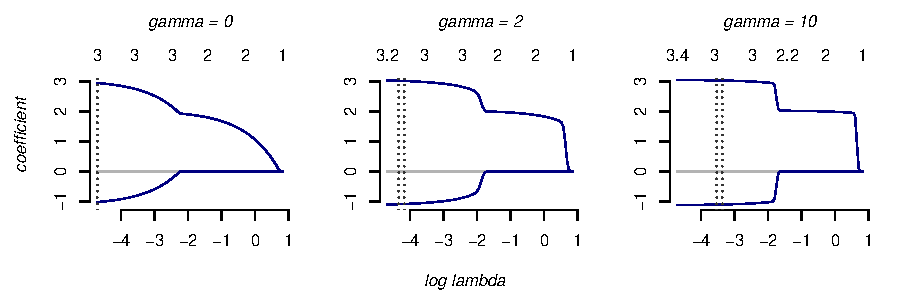
\includegraphics[width=6.5in]{gamlr_eg}
\vskip -.25cm
\caption{\label{gamlr_eg} Gamma lasso estimation on $n=10^3$ 
 observations of $y_i = 4 + 3x_{1i} - x_{2i} + \varepsilon_i$, where
$\varepsilon_i \stackrel{ind}{\sim} \mr{N}(0,1)$ and
$\{x_{1i},x_{2i},x_{3i}\}$ are marginally standard normal with correlation of
0.9 between covariates ($x_{3i}$ is spurious). The penalty path has $T=100$
segments, $\lambda^1 = n^{-1}\left| \sum_i x_{1i}y_i\right|$, and
$\lambda^{100} = 0.01\lambda^1$. Degrees of freedom are on top and vertical
lines mark AICc and BIC selected models (see Section
\ref{sss}).}
\vskip -.25cm
\end{figure}

Each  gamma lasso path segment is solved through coordinate descent,
as detailed in Appendix \ref{implement}.  The algorithm is implemented in {\tt
c} as part of the {\tt gamlr} package for {\sf R}. The software  has detailed documentation and versioned source code is at
{\tt github.com/mataddy/gamlr}.  Usage of {\tt gamlr} mirrors that of its
convex penalty analogue {\tt glmnet} \citep{friedman_regularization_2010}, the
fantastic and widely used package for costs between $L_1$ and $L_2$ norms. In
the lasso case ($\gamma=0$), the two algorithms are essentially equivalent.


\subsection{Bayesian motivation}

Consider a model where each $\beta_j$ is
assigned a Laplace distribution prior with scale $\tau_j>0$,
\begin{equation}\label{blasso}
\beta_j \sim \mr{La}\left(\tau_j\right) =
\frac{\tau_j}{2}\exp\left[ -\tau_j|\beta_j| ~\right].
\end{equation}
Typically, scale parameters $\tau_1 =
\ldots = \tau_p$ are set as a single shared value, say $n\lambda/\phi$ where
 $\phi$ is the exponential family dispersion (e.g. Gaussian variance
$\sigma^2$ or 1 for the binomial).   Posterior
maximization under the prior in (\ref{blasso}) is then lasso estimation \citep[e.g.,][]{park_bayesian_2008}.

Instead of working from shared scale, assume an independent gamma
$\mr{Ga}(s,1/\gamma)$ hyperprior with `shape' $s$ and `scale' $\gamma$ for
each $\tau_j$, such that $\ds{E}[\tau_j] = s\gamma$ and $\mr{var}(\tau_j) =
s\gamma^2$.  Then the {\it joint} prior for both coefficient and scale is
\begin{equation}\label{glprior}
\pi(\beta_j,\tau_j) = \mr{La}\left(\beta_j ;~ \tau_j\right)
\mr{Ga}\left(\tau_j;~ s,\gamma^{-1}\right) = \frac{ 1}{2\Gamma({s})} 
\left(\frac{\tau_j}{\gamma}\right)^{s}
               \exp\left[-\tau_j(\gamma^{-1}+|\beta_j|)\right].
\end{equation}
The gamma hyperprior is conjugate here, implying a $\mr{Ga}\left(s+1, ~1/\gamma +
|\beta_j|\right)$ posterior for $\tau_j \mid \beta_j$ with conditional
posterior mode (MAP) at $\hat\tau_j = \gamma s/(1 + \gamma |\beta_j|)$.

Consider joint MAP estimation of $[\bs{\tau},\bs{\beta}]$ under the prior in
   (\ref{glprior}), where we've suppressed $\alpha$ for simplicity. By taking
   negative logs and removing constants, this is equivalent to solving
\begin{equation}\label{gljoint}
\min_{\beta_j\in\ds{R},~\tau_j \in \ds{R}^{+}}~~
\phi^{-1}l(\bs{\beta}) + \sum_j \left[\tau_j(\gamma^{-1}+|\beta_j|) - s\log(\tau_j)\right].
\end{equation}
It is straightforward to show that (\ref{gljoint}) is equivalent 
to the log-penalized objective 
\begin{equation}\label{logobj}
\min_{\beta_j\in\ds{R}}~~
\phi^{-1}l(\bs{\beta}) + \sum_j  s\log(1+\gamma|\beta_j|)
\end{equation}

\begin{prop}\label{penprop}
  $\bs{\hat\beta}$ solves (\ref{logobj}) if and only if it is also in the
  solution to (\ref{gljoint}).
\end{prop}
\begin{proof}
  The conditional posterior mode for each $\tau_j$ given $\beta_j$
  is $\tau(\beta_j) = \gamma s/(1 + \gamma|\beta_j|)$.  Any joint solution
  $[\bs{\hat\beta},\bs{\hat\tau}]$ for (\ref{gljoint}) thus
  consists of $\hat{\tau}_{j} = \tau(\hat\beta_{j})$;
  otherwise, it is always possible to decrease the objective by
  replacing $\hat\tau_{j}$. Setting each $\tau_j = 
  \tau(\beta_j)$ in (\ref{gljoint}) and removing constant terms yields
  (\ref{logobj}).  Moreover, the solution to (\ref{gljoint}) solves
  (\ref{logobj}): otherwise, there would need to be a point on the profile
  slice of (\ref{gljoint}) defined by $\tau_{j} =
  \tau(\hat\beta_{j})$ that is lower than its minimum.
\end{proof}

For a Bayesian it is odd to be solving for $\bs{\tau}$ rather than
marginalizing over its uncertainty.  However, recognizing the form of a gamma
density  in (\ref{glprior}), $\pi(\beta_j,\tau_j)$ integrates over $\tau_j$ to
yield the marginal prior $ \pi(\beta_j) = 0.5s\left( 1+
\gamma|\beta_j|\right)^{-(s+1)}$. This is the generalized double Pareto
density, as in  \citet{armagan_generalized_2013}. Since $-\log \pi(\beta_j)
\propto (s+1)\log(1 + \gamma|\beta_j|)$, the {\it profile} MAP solution to
(\ref{gljoint}) is also the {\it marginal} MAP for
$\bs{\beta}$ under $\mr{Ga}(s-1,1/\gamma)$ priors on each $\tau_j$.


\section{Speed, stability, and selection}
\label{sss}


As we've mentioned repeatedly, the lasso, POSE, GL and related techniques from
sparse regularization do not actually {\it do} model selection; rather, the
paths of estimators corresponding to different levels of penalization provide
a set of candidates from which one must choose. It is essential that these
paths are quick to obtain and are good platforms for model selection.

The lasso has become hugely popular because its path solutions have both of
these properties.  Diminishing bias extensions, such as GL, can provide
improved prediction and information compression over the lasso in many
settings.  However, when the bias diminishes too quickly (e.g., for $\gamma$
too large), the paths become {\it instable}. For example, consider exact (not
GL) solutions under the log penalty as plotted in Figure \ref{solution}: the
minimizer of the solid line of the right panel  will jump from 0 to 3.5
depending upon small jitter either to data $B$ or cost $\gamma s$.  Such
instability costs us in two ways.\footnote{For a classic article on the issues
of model instability, see \citet{breiman_heuristics_1996}.}
\begin{itemize}
\item Computation becomes expensive:
the coefficients change quickly, or even jump, along the path and are no
longer good hot-starts for the next segment.
\item Model selection becomes difficult:  estimates are sensitive to 
small amount of data jitter, so that the variability explodes for any choice
based upon these estimates.
\end{itemize}
This section reviews balance between the benefits of diminishing-bias and
the dangers of instability, working through concrete guidelines for
application of the GL algorithm.

\subsection{Stability}

A strong form of stability comes from convexity of the penalized objective in
(\ref{pendev}). This requires that the minimum eigenvalue of
$\bm{H}(\bs{\beta})$, the Hessian matrix of second derivatives of
$l(\bs{\beta})$, is greater than $|c''(\beta_j)| ~\forall j$.  For penalized
least-squares under log costs, this amounts to requiring that the minimum
eigenvalue of $\bm{H} = \bm{X}'\bm{X}$ is greater than
$\lambda\gamma^2$.\footnote{ If $\nu$ is an eigenvalue of $\bm{H}$, then
$(\bm{H} -
\nu \bm{I})\bm{v} = 0$ for some nonzero $\bm{v}$; the negative log posterior
Hessian at zero is $\bm{H} - \lambda\gamma^2\bm{I}$ and $(\bm{H} -
\lambda\gamma^2\bm{I} + s\gamma^2\bm{I} -
\nu \bm{I})\bm{v} = 0$ so that 
$\nu - s\gamma^2$ is an eigenvalue of the minimization objective.  }  In the
simple {\it standardized orthogonal covariate} case, this has an easy
interpretation in the context of our Bayesian model from Section \ref{pose}.2:
for Gaussian regression, $h_j = \sum_i x_{ij}^2 = n$ and the objective is
convex if prior variance on each $\tau_j$  is less than the number of
observations.  For logistic regression you need $\mr{var}(\tau_j) < n/4$,
since $\bm{H}$ now depends upon the coefficient values.

In real examples, however, we cannot rely upon objective convexity. A more
useful definition of stability requires continuity of the implied  coefficient
function, $\hat\beta(\bm{y})$, in an imagined univariate regression problem
(or for orthogonal covariates).  This is one of the key requirements of
concave penalties listed by \citet{fan_variable_2001}. Many popular concave
cost functions, such as the SCAD and MCP, have been engineered to have this
continuity property. Conveniently, \cite{zou_one-step_2008} show that OSE LLA
solutions have this property even if the target objective does not.  For
example, even though the log penalty {\it does not} generally lead to
continuous thresholding, their result implies that the GL solutions are
continuous for $\gamma<\infty$.

A theoretically richer form of stability is Lipschitz continuity of the
implied prediction function, $\boldsymbol{\hat y} = \bm{X}\boldsymbol{\hat
\beta}(\bm{y})$, which requires that   $
\|\bm{\hat y}(\bm{y}_1)-\bm{\hat y}(\bm{y}_2)| \leq L\|\bm{y}_1-\bm{y}_2\| $
for some finite constant $L$ on all possible $\bm{y}_1,\bm{y}_2$.
\citet{zou_degrees_2007} establish Lipschitz continuity for $L_1$ estimated
predictors as part of their derivation of a degrees-of-freedom estimator.
Thus, conditional upon values for the coefficient-specific weights, POSE and
GL are trivially Lipschitz continuous.  Unconditionally, we do not believe
that the paths have this guarantee.  However, we'll see in the next section
that a heuristic degrees-of-freedom estimator that takes such stability for
granted performs well as the basis for model selection.

Finally, the basic and most important type of stability is practical path continuity: by this, we mean that solutions change slowly enough along the path so that computational costs are kept within budget.   A regularization path can be built from a continuous thresholding function, or perhaps even be Lipschitz stable, but 
none of that matters if it takes too long to fit.  For example, Figure \ref{nhltime} shows timings growing rapidly with large $\gamma$ for the hockey data  of Section \ref{eg}.2, even though all of these specifications are theoretically stable by some criteria.

\begin{figure}[bht]
\vskip -.5cm
\centering
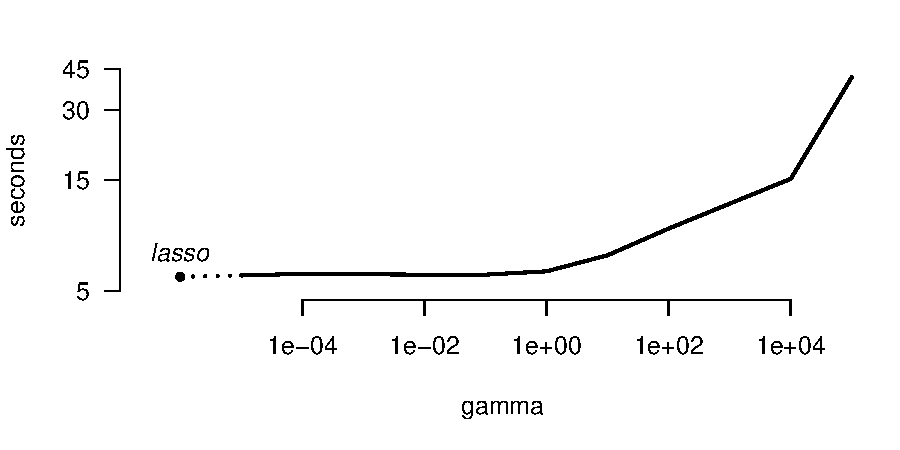
\includegraphics[width=5in]{nhl_time}
\vskip -.25cm
\caption{\label{nhltime} 
Timings for the hockey data path fits of Section \ref{eg}.2
on a length-100 grid with $\lambda^{100} = 0.01\lambda^1$. }
\vskip -.25cm
\end{figure}


\subsection{Selection}


We would like to choose a model that performs well in predicting new data.
 `Good prediction' can be measured in a variety of ways.  A common and
 coherent framework is to consider minimizing Kullback-Leibler (KL)
 divergence.  Say $g(\bm{y})$ is the true data generating process, and
 $f(\bm{y}; \bs{\eta},\phi)$ is the parametric density under study, which we
 suppose here is a natural exponential family  with $\ds{E}[\bm{y}]=\bs{\eta}$
 and dispersion $\phi$. Then we wish to minimize
\begin{equation}
\mr{KL}(\bs{\eta},\phi) = \ds{E}_g \log g(\bm{y}) - \ds{E}_g \log f(\bm{y}; \bs{\eta},\phi),
\end{equation}
the expected difference between log true density and our parametric approximation.  Since $\ds{E}_g \log g(\bm{y})$ is constant, this leads one to minimize 
$Q(\bs{\eta},\phi) = -\ds{E}_g \log f(\bm{y}; \bs{\eta},\phi)$, the expected negative log likelihood.   There is no requirement that $g$ is a member of the family defined by $f$.

If parameters are to be estimated as $[\bs{\eta}_{\bm{y}},\phi_{\bm{y}}]$, functions of random sample $\bm{y} \sim g$, then $Q(\bs{\eta}_{\bm{y}},\phi_{\bm{y}})$ is itself a random variable and one chooses estimators to minimize its expectation.  {\it Crucially, we imagine a double-sample expectation}, where the minimization objective is
\begin{equation}\label{dualexpect}
\ds{E}_{\bm{y}|g} \ds{E}_{\bm{\tilde y}|g} \log f(\bm{\tilde y}; \bs{\eta}_{\bm{y}},\phi_{\bm{y}}).
\end{equation}
The notation here indicates that inner and outer expectations are based on two {\it independent} random samples from $g$: $\bm{y}$ for training, upon which $\bs{\eta}_{\bm{y}},\phi_{\bm{y}}$ are calculated, and $\bm{\tilde y}$ for validation.  

The remainder of this section outlines two strategies for minimization of (\ref{dualexpect}).  The first, cross-validation, performs a Monte Carlo experiment that mimics double expectation.  The second set of methods, information criteria, attempt to approximate (\ref{dualexpect}) analytically via the observed likelihood and a complexity penalty that depends upon the degrees of freedom.

\subsubsection{Cross validation}
\label{cv}

$K$-fold cross-validation \cite[CV; see][for an
overview]{efron_estimation_2004} estimates the double expectation in
(\ref{dualexpect}) through a simple experiment: split the sample $\mc{S} =
\{\bm{x}_i,y_i\}_{i=1}^n$ into $K$  disjoint subsets (folds) $\mc{S}_k$,
and $K$ times fit a regularization path given $\mc{S} \setminus \mc{S}_k$ and
use this to predict on $\mc{S}_k$.  This yields $K$  realizations of
`out-of-sample' (OOS) deviance, and you averaged across folds to get an
estimate for (\ref{dualexpect}) along the along the regularization path. One then selects $\lambda$ according to some criterion and re-fits the
model on the entire dataset under this penalty.  The usual rules are either
CV.min, choose the $\lambda$ with minimum average OOS error, or
CV.1se, choose the largest $\lambda$ with mean OOS error no more than
1 standard error away from the minimum. 

CV is super useful, and some form of it features in most applications, but it
does have some weaknesses. If a single fit is expensive then doing it $K$
times will be impractical.  More subtly, truly Big data are distributed: they
are too large to store on a single machine. Algorithms can be designed to work
in parallel on subsets
\citep[e.g.,][]{taddy_distributed_2013}, but a bottleneck
results if you need to communicate across machines for OOS experimentation.
Finally, large organizations may wish to avoid the
Monte Carlo error of CV -- they'll want the same answer every time.  Thus it
is useful to have an analytic estimator for (\ref{dualexpect}) that requires only  a single model fit.


\subsubsection{Information Criteria: AIC and AICc}


Information criteria (IC) are analytic approximations to metrics like
(\ref{dualexpect}).\footnote{Not all IC target (\ref{dualexpect}).  For
example, the `Bayesian' BIC, with  $c(df) =\log(n)df$
\citep{schwarz_estimating_1978}, is derived
\citep{kass_bayes_1995} as Laplace approximation to the negative log of the
 {\it marginal likelihood}.  We include the BIC as a comparator to AIC and
 AICc in our examples. }  They take the form
\begin{equation}\label{ic}
 -2\log f(\bm{y}; \bs{\eta}_{\bm{y}},\phi_{\bm{y}}) + c(df)
 \end{equation} 
where $c(df)$ is cost of the {\it degrees-of-freedom} used in
$\bs{\eta}_{\bm{y}}$ -- e.g., for $\bm{y} \sim (\bs{\eta},\sigma^2\bm{I})$,
\citet{efron_least_2004} defines $df =
\sigma^{-2} \sum_i \mr{cov}(\eta_{\bm{y}i}, y_i)$. 


The commonly applied AIC uses $c(df)=2df$ and is derived as an asymptotic approximation to (\ref{dualexpect}) in 
\cite{akaike_information_1973}.  However, our experience (e.g., see Section
\ref{eg}.1) is that AIC selects over-fit models when applied to high dimensional
problems.  This is because the approximation upon which it is based
is valid only for large $n/df$ \citep{burnham_model_2002}.  A `corrected' AICc
for finite $n/df$ is derived in
\cite{hurvich_regression_1989}, and \citet{flynn_efficiency_2013} study its
application to penalized deviance estimation.
\begin{equation}
\text{AICc:}~~~-2\log f(\bm{y}; \bs{\eta}_{\bm{y}},\phi_{\bm{y}}) + 2df\frac{n}{n-df-1}.
\end{equation}
The correction multiplier is $n/(n-df-1)$, and AICc approaches standard AIC if
$n\gg df$. See Appendix \ref{aicder} for a simple derivation of the AICc in
linear models, \cite{claeskens_model_2008} for a more traditional derivation
and full theoretical review of information criteria, and refer to
\citet{flynn_efficiency_2013} for results extending to generalized linear
models.

In order to make use of the AICc or AIC, we need to have a value for the
number of degrees-of-freedom. In an unpenalized linear model, $df$ is just the
number of coefficients.   For some penalization schemes, such as the original
least-squares lasso
\citep{zou_degrees_2007}, unbiased estimates for $df$ are available
analytically.   More generally, it is common to rely upon heuristic arguments
(e.g., even for lasso penalized logistic regression we are unaware of
theoretically unbiased estimators).  A heuristic is what we'll propose here.

For prediction rules that are suitably stable \citep[i.e., Lipschitz; see][]{zou_degrees_2007}, the SURE framework of
\cite{stein_estimation_1981} applies and we get the relatively
easy-to-work-with expression  $df =
\ds{E}\left[\sum_i \partial \eta_{\bm{y}i}/\partial y_i\right]$.
Consider  a single coefficient $\beta$ estimated via least-squares under $L_1$
penalty $\tau$.   Write gradient at zero $g = -\sum_i x_iy_i$ and curvature $h
= \sum_i x_i^2$ and set $\varsigma = -{\tt sign}(g)$. The prediction rule is
$\eta_{\bm{y}} = x(\varsigma/h)(|g|-\tau)_+$ with  derivative $\partial \eta_{\bm{y}i}/\partial y = x_i^2/h \ds{1}_{[|g|<\tau]}$, so that the SURE expression
yields $df = \ds{E}\left[ \ds{1}_{[|g|<\tau]} \right]$.   This expectation is
taken with respect to the {\it unknown true} distribution over $\bm{y} |
\bm{X}$, not that estimated from the observed sample.  However, as an estimator
\citep[e.g.,][]{zou_degrees_2007} one can evaluate this expression at observed
gradients.

This motivates our heuristic $df$ in weighted $L_1$ regularization:  the {\it prior} expectation for the number  $L_1$ penalty dimensions, $\tau_j = \lambda \omega_j$, that are less than their corresponding absolute gradient dimension.  Referring back to the Bayesian model of Section \ref{pose}.2, each $\tau_j$ is IID $\mr{Ga}(s,1/\gamma)$ in the prior,
leading to the {\it gamma lasso estimator for degrees of freedom}\footnote{The number of unpenalized coefficients (e.g.,~1 for
$\alpha$) is always added to this to get total $df$.} 
\begin{equation}
\label{edf} df^t = \sum_j \mr{Ga}(|g_{j}|;~n\lambda^t/(\gamma\phi),
1/\gamma), \end{equation} where $\mr{Ga}(~\cdot~;~\mr{shape}, 1/\mr{scale})$
is the Gamma distribution function and $g_j$ is an estimate of  the
$j^{th}$ coefficient gradient evaluated at $\hat\beta_j=0$.  For fully orthogonal covariates,  $g_j$ is available as the marginal gradient at zero.
In the non-orthogonal case, where $g_{j} = g_j(0)$ becomes a
function of all of the elements of $\bs{\hat\beta}$, we plug in the most recent
$g_j$ at which $\hat\beta^t_j=0$:  this
requires no extra computation and has the advantage of maintaining $df =
\hat p^t$ for $\gamma = 0$.

The $df$ estimator in (\ref{edf}) seems intuitively reasonable; for example,
$\lim_{\gamma \to 0} df^t = \hat p^t$ and  $\lim_{\gamma \to \infty} df^t= p$.
However, the derivation is purely heuristic and we rely on empirical results to
justify its application as part of an AICc criteria.  When used as an input
to AICc, as in the next section, it allows those criteria to perform as well
or better than nonparametric cross-validation.

\section{Examples}
\label{eg}

\subsection{Simulation}

This section will  analyze data simulated from
 the following $p=1000$ dimensional regression.
\begin{align}
\label{simdgp}
y \sim \mr{N}\left(\bm{x}'\bs{\beta},\sigma^2\right)~~\text{where}~~\bm{x} = \bm{u}*\bm{z},~~\bm{x}\sim \mr{N}\left(\bm{0},\bs{\Sigma}\right),~~z_{j} \stackrel{ind}{\sim} \mr{Bin}(0.5),~~\beta_j = \frac{1}{j}\exp\left(-\frac{j}{50}\right).
\end{align}

\vspace{-.4cm}
\noindent
Each simulation draws $n=1000$ means $\eta_i =
\bm{x}_i'\bs{\beta}$, and two independent response samples 
$\bm{y},\bm{\tilde y} \sim \mr{N}(\bs{\eta},\sigma^2\bm{I})$. Residual
variance $\sigma^2$ and covariate correlation $\bs{\Sigma}$ are adjusted across
runs.  In the first case, we define $\sigma^2$ through {\it signal-to-noise}
ratios $\mr{sd}(\bs{\eta})/\sigma$ of $1/2$, $1$, and $2$.  In the latter
case, multicollinearity is parametrized via $\Sigma_{jk} =
\rho^{|j-k|}$, and we consider $\rho = 0, 0.5,~\text{and}~0.9$.


The regression in (\ref{simdgp}) is obviously {\it dense}:  true
coefficients are all nonzero.  However, they decay in magnitude along the
index $j$ and
it will be useless to estimate many of them in a $p=n$ regression.
Our sparse oracle comparator is the $C_p$ optimal $L_0$ penalized solution

\vspace{-.3cm}
\begin{equation}\label{l0oracle}
\bs{\beta}^{\star} = \argmin_{\bs{\beta}} \left\{ \|\bm{y}-\bm{X}\bs{\beta}\|^2 + 2\sigma^2\sum_j
\ds{1}_{\{\beta_j\neq0\}}\right\},
\end{equation} which is solvable here by searching through
OLS regression on $\bm{X}_{\{1\ldots j\}}$ for $j=1\ldots p$.

We consider {\tt gamlr} runs of GL with $\gamma$
of 0 (lasso), 2, and 10 and marginal AL, as well as
{\tt sparsenet}'s MCP penalized regression.  Covariate penalties are
standardized by $\mr{sd}(\bs{x}_j)$, and paths run through 100
$\lambda$ values down to $\lambda^{100} = 0.01\lambda^1$. On an Intel Xeon
E5-2670 core, 5-fold CV with $\mr{sd}(\bm{\eta})/\sigma=1$
and $\rho=1/2$ requires   1-2 seconds for lasso and marginal  AL, 2 and 3
seconds for GL with $\gamma=2$ and $\gamma=10$, and 15-20 seconds
for Sparsenet.
\footnote{{\tt ncvreg} SCAD required ten minutes for a single run and is thus
impractical for the applications under consideration.  But, in a small study,
CV.min selected SCAD performs quite well in prediction --  similarly to the
best CV.min methods for each data configuration -- with relatively high values
for both false discovery and sensitivity. }


Figures \ref{simpaths} and \ref{simcv} illustrate GL paths for a single
dataset, with  $\mr{sd}(\bm{\eta})/\sigma=1$ and $\rho=1/2$. In Figure
\ref{simpaths}, increasing $\gamma$ leads to `larger shouldered' paths where
estimates move quickly to MLE for the nonzero-coefficients. Degrees of
freedom, calculated as in (\ref{edf}), are along the top of each plot; equal
$\lambda$ have higher $df^t$ for higher $\gamma$ since there is less shrinkage
of $\hat\beta_j\neq0$.  Figure \ref{simcv} shows CV and AICc error estimates.
The two criteria roughly track each other, although AICc more heavily
penalizes over-fit and at $\gamma=10$ their minima do not match.  Notice that
as $\gamma$ increases, the CV error increases more quickly after it's minimum;
this indicates that the consequences of over-fit are worse under faster
diminishing-bias.


\begin{figure}[tb]
{\small \hskip 2.5cm$\bs{\gamma=0}$\hskip 4cm$\bs{\gamma=2}$\hskip 4cm$\bs{\gamma=10}$}

~~~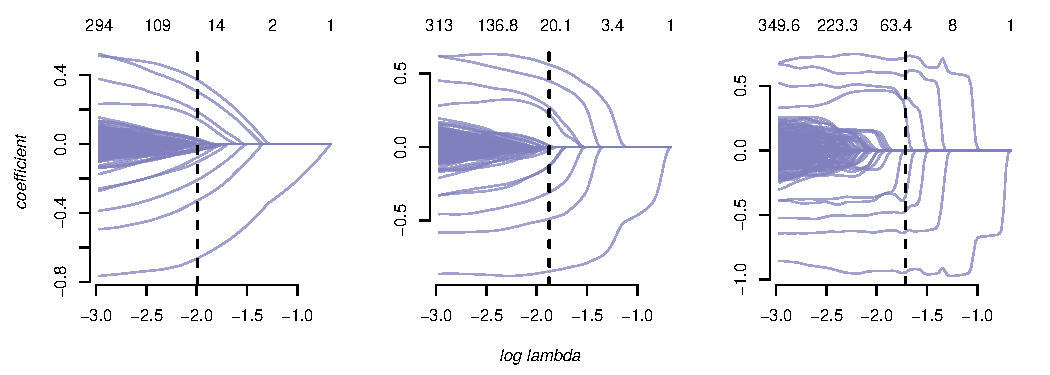
\includegraphics[width=6in]{sim_paths}
\caption{\label{simpaths} Regularization paths for simulation example.
Degrees of freedom $df^t$ are along the top. }
\vskip .3cm
{\small \hskip 2.5cm$\bs{\gamma=0}$\hskip 4cm$\bs{\gamma=2}$\hskip 4cm$\bs{\gamma=10}$}

~~~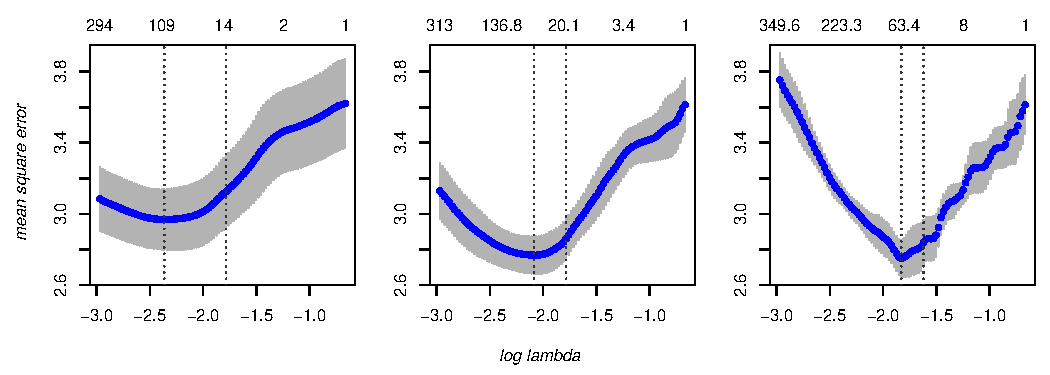
\includegraphics[width=6in]{sim_cv}
\caption{\label{simcv} 5-fold CV and AICc for a simulation example. 
Points-and-bars show mean OOS MSE $\pm 1$se.  }
\vspace{-.25cm}
\end{figure}

% \begin{table}[p]\vspace{-.5cm}
% \caption[l]{\it Predictive Mean Square Error\hfill}
% \vspace{-.5cm}
% \small\setstretch{1}
% \begin{center}
% \begin{tabular}{l*{5}{c}|r}
%  & lasso & GL $\gamma=2$ & GL $\gamma=10$ & marginal AL & sparsenet MCP  &  \\
% \cline{1-7}
% CV.1se & 4.4 & 4.3 & 4.8 & 4.3 & 4.2 &\\
% CV.min & 4.1 & {\bf 4} & 4.3 & 4.1 & {\bf 4} &  $\mr{sd}(\bm{\mu})/\sigma=2$ \\
% AICc & 4.3 & 4.1 & 4.1 & 4.2 & & $\rho=0$ \\
% AIC & 5 & 5.2 & 5.2 & 4.1 & & \multirow{2}{*}{$C_p$ mse = 3.5} \\
% BIC & 5.6 & 5.1 & 5.7 & 4.9 & & \\
%  \hline 
% CV.1se & 3.1 & 3 & 3.4 & 3.1 & 2.9 &\\
% CV.min & 2.9 & {\bf 2.8} & 3 & 3 & {\bf 2.8} &  $\mr{sd}(\bm{\mu})/\sigma=2$ \\
% AICc & 3 & {\bf 2.8} & 2.9 & 3 & & $\rho=0.5$ \\
% AIC & 3.4 & 3.5 & 3.5 & 2.9 & & \multirow{2}{*}{$C_p$ mse = 2.4} \\
% BIC & 4.4 & 3.7 & 4.1 & 3.8 & & \\
%  \hline 
% CV.1se & 2.4 & 2.4 & 2.6 & 2.6 & 2.3 &\\
% CV.min & 2.3 & {\bf 2.2} & 2.3 & 2.4 & {\bf 2.2} &  $\mr{sd}(\bm{\mu})/\sigma=2$ \\
% AICc & 2.4 & {\bf 2.2} & 2.3 & 2.5 & & $\rho=0.9$ \\
% AIC & 2.6 & 2.7 & 2.7 & 2.4 & & \multirow{2}{*}{$C_p$ mse = 1.9} \\
% BIC & 3.5 & 3 & 3.3 & 3.2 & & \\
%  \hline 
% CV.1se & 17 & 16.9 & 18 & 15.6 & 16.4 &\\
% CV.min & 15.6 & 15.6 & 16.5 & 15.7 & 15.6 &  $\mr{sd}(\bm{\mu})/\sigma=1$ \\
% AICc & 15.8 & {\bf 15.5} & 15.9 & 15.6 & & $\rho=0$ \\
% AIC & 21.3 & 22.2 & 22.2 & 17 & & \multirow{2}{*}{$C_p$ mse = 13.8} \\
% BIC & 20.8 & 19.2 & 23.4 & 17.7 & & \\
%  \hline 
% CV.1se & 12 & 11.7 & 12.7 & 11.1 & 11.3 &\\
% CV.min & 10.9 & 10.8 & 11.5 & 11 & 10.8 &  $\mr{sd}(\bm{\mu})/\sigma=1$ \\
% AICc & 11.1 & {\bf 10.7} & 10.8 & 11 & & $\rho=0.5$ \\
% AIC & 14.4 & 14.9 & 14.9 & 11.8 & & \multirow{2}{*}{$C_p$ mse = 9.2} \\
% BIC & 15.8 & 14.4 & 16.1 & 13.4 & & \\
%  \hline 
% CV.1se & 9.4 & 9.2 & 10.1 & 9.1 & 8.9 &\\
% CV.min & 8.6 & {\bf 8.5} & 9 & 8.8 & {\bf 8.5} &  $\mr{sd}(\bm{\mu})/\sigma=1$ \\
% AICc & 8.8 & {\bf 8.5} & {\bf 8.5} & 8.8 & & $\rho=0.9$ \\
% AIC & 11.2 & 11.6 & 11.6 & 9.1 & & \multirow{2}{*}{$C_p$ mse = 7.3} \\
% BIC & 12.7 & 12.1 & 12.9 & 11.4 & & \\
%  \hline 
% CV.1se & 60.9 & 61.2 & 61.3 & 57.8 & 61 &\\
% CV.min & 57.8 & 59.8 & 60.6 & 60.5 & 57.9 &  $\mr{sd}(\bm{\mu})/\sigma=0.5$ \\
% AICc & {\bf 57.6} & 60 & 61.4 & 59 & & $\rho=0$ \\
% AIC & 88.4 & 92.5 & 92.5 & 73.2 & & \multirow{2}{*}{$C_p$ mse = 53.5} \\
% BIC & 61.3 & 61.3 & 61.3 & 60.6 & & \\
%  \hline 
% CV.1se & 41.1 & 41.2 & 41.2 & 39.8 & 41.2 &\\
% CV.min & 39.9 & 40.7 & 41 & 41.3 & 39.9 &  $\mr{sd}(\bm{\mu})/\sigma=0.5$ \\
% AICc & {\bf 39.6} & 40.5 & 41.3 & 40.5 & & $\rho=0.5$ \\
% AIC & 59.4 & 61.9 & 61.9 & 49.9 & & \multirow{2}{*}{$C_p$ mse = 35.9} \\
% BIC & 41.2 & 41.2 & 41.2 & 41 & & \\
%  \hline 
% CV.1se & 32.6 & 32.6 & 32.6 & 31.8 & 32.6 &\\
% CV.min & 31.8 & 32.3 & 32.5 & 32.4 & 31.8 &  $\mr{sd}(\bm{\mu})/\sigma=0.5$ \\
% AICc & {\bf 31.5} & 32.1 & 32.6 & 32.2 & & $\rho=0.9$ \\
% AIC & 46.4 & 48.6 & 48.6 & 38.1 & & \multirow{2}{*}{$C_p$ mse = 28.3} \\
% BIC & 32.6 & 32.6 & 32.6 & 32.5 & & \\
%  \hline \end{tabular}
% \end{center}
% \vspace{-1cm}
% \end{table}

\begin{table}[p]\vspace{-.5cm}
\caption[l]{\label{r2}\it Predictive $R^2$\hfill}
\vspace{-.5cm}
\small\setstretch{1}
\begin{center}
\begin{tabular}{l*{5}{c}|r}
 & lasso & GL $\gamma=2$ & GL $\gamma=10$ & marginal AL & sparsenet MCP  &  \\
\cline{1-7}
CV.1se & 0.71 & 0.72 & 0.68 & 0.72 & 0.73 &\\
CV.min & 0.73 & {\bf 0.74} & 0.72 & 0.73 & {\bf 0.74} &  $\mr{sd}(\bm{\mu})/\sigma=2$ \\
AICc & 0.72 & 0.73 & 0.73 & 0.73 & & $\rho=0$ \\
AIC & 0.67 & 0.66 & 0.66 & 0.73 & & \multirow{2}{*}{$C_p ~ R^2$ = 0.77} \\
BIC & 0.63 & 0.67 & 0.63 & 0.68 & & \\
 \hline 
CV.1se & 0.7 & 0.71 & 0.67 & 0.7 & 0.72 &\\
CV.min & 0.72 & {\bf 0.73} & 0.7 & 0.71 & {\bf 0.73} &  $\mr{sd}(\bm{\mu})/\sigma=2$ \\
AICc & 0.71 & {\bf 0.73} & 0.72 & 0.71 & & $\rho=0.5$ \\
AIC & 0.67 & 0.66 & 0.66 & 0.71 & & \multirow{2}{*}{$C_p ~ R^2$ = 0.77} \\
BIC & 0.57 & 0.64 & 0.6 & 0.63 & & \\
 \hline 
CV.1se & 0.7 & 0.71 & 0.68 & 0.68 & 0.72 &\\
CV.min & 0.72 & {\bf 0.73} & 0.71 & 0.7 & {\bf 0.73} &  $\mr{sd}(\bm{\mu})/\sigma=2$ \\
AICc & 0.71 & {\bf 0.73} & 0.72 & 0.7 & & $\rho=0.9$ \\
AIC & 0.68 & 0.67 & 0.67 & 0.7 & & \multirow{2}{*}{$C_p ~ R^2$ = 0.77} \\
BIC & 0.57 & 0.63 & 0.6 & 0.61 & & \\
 \hline 
CV.1se & 0.31 & 0.31 & 0.27 & 0.36 & 0.33 &\\
CV.min & 0.36 & 0.36 & 0.33 & 0.36 & 0.36 &  $\mr{sd}(\bm{\mu})/\sigma=1$ \\
AICc & 0.35 & {\bf 0.37} & 0.35 & 0.36 & & $\rho=0$ \\
AIC & 0.13 & 0.09 & 0.09 & 0.3 & & \multirow{2}{*}{$C_p ~ R^2$ = 0.44} \\
BIC & 0.15 & 0.22 & 0.04 & 0.28 & & \\
 \hline 
CV.1se & 0.27 & 0.29 & 0.23 & 0.33 & 0.32 &\\
CV.min & 0.34 & {\bf 0.35} & 0.3 & 0.33 & {\bf 0.35} &  $\mr{sd}(\bm{\mu})/\sigma=1$ \\
AICc & 0.32 & {\bf 0.35} & {\bf 0.35} & 0.33 & & $\rho=0.5$ \\
AIC & 0.12 & 0.1 & 0.1 & 0.28 & & \multirow{2}{*}{$C_p ~ R^2$ = 0.44} \\
BIC & 0.04 & 0.13 & 0.02 & 0.19 & & \\
 \hline 
CV.1se & 0.28 & 0.29 & 0.23 & 0.3 & 0.31 &\\
CV.min & 0.34 & {\bf 0.35} & 0.31 & 0.32 & {\bf 0.35} &  $\mr{sd}(\bm{\mu})/\sigma=1$ \\
AICc & 0.33 & {\bf 0.35} & {\bf 0.35} & 0.32 & & $\rho=0.9$ \\
AIC & 0.14 & 0.11 & 0.11 & 0.3 & & \multirow{2}{*}{$C_p ~ R^2$ = 0.44} \\
BIC & 0.03 & 0.07 & 0.01 & 0.13 & & \\
 \hline 
CV.1se & 0.01 & 0 & 0 & {\bf 0.06} & 0 &\\
CV.min & {\bf 0.06} & 0.02 & 0.01 & 0.01 & 0.05 &  $\mr{sd}(\bm{\mu})/\sigma=0.5$ \\
AICc & {\bf 0.06} & 0.02 & 0 & 0.04 & & $\rho=0$ \\
AIC & -0.44 & -0.51 & -0.51 & -0.2 & & \multirow{2}{*}{$C_p ~ R^2$ = 0.13} \\
BIC & 0 & 0 & 0 & 0.01 & & \\
 \hline 
CV.1se & 0 & 0 & 0 & 0.03 & 0 &\\
CV.min & 0.03 & 0.01 & 0 & -0.01 & 0.03 &  $\mr{sd}(\bm{\mu})/\sigma=0.5$ \\
AICc & {\bf 0.04} & 0.01 & 0 & 0.01 & & $\rho=0.5$ \\
AIC & -0.45 & -0.51 & -0.51 & -0.21 & & \multirow{2}{*}{$C_p ~ R^2$ = 0.13} \\
BIC & 0 & 0 & 0 & 0 & & \\
 \hline 
CV.1se & 0 & 0 & 0 & 0.02 & 0 &\\
CV.min & 0.02 & 0.01 & 0 & 0 & 0.02 &  $\mr{sd}(\bm{\mu})/\sigma=0.5$ \\
AICc & {\bf 0.03} & 0.01 & 0 & 0.01 & & $\rho=0.9$ \\
AIC & -0.43 & -0.5 & -0.5 & -0.17 & & \multirow{2}{*}{$C_p ~ R^2$ = 0.13} \\
BIC & 0 & 0 & 0 & 0 & & \\
 \hline 
\end{tabular}
\end{center}
\vspace{-1cm}
\end{table}

\begin{table}[p]\vspace{-.5cm}
\caption[l]{\label{sens}\it False Discovery Rate $\mid$ Sensitivity, relative to $C_p$ model\hfill}
\vspace{-.5cm}
\small\setstretch{1}
\begin{center}
\begin{tabular}{l*{5}{c}|r}
 & lasso & GL $\gamma=2$ & GL $\gamma=10$ & marginal AL & sparsenet MCP  & \\
 \cline{1-7}
CV.1se & 0.49 $\mid$ 0.76 & 0.26 $\mid$ 0.67 & 0.07 $\mid$ 0.56 & 0.43 $\mid$ 0.67 & 0.15 $\mid$ 0.61 &\\
CV.min & 0.65 $\mid$ 0.84 & 0.48 $\mid$ 0.77 & 0.20 $\mid$ 0.65 & 0.57 $\mid$ 0.74 & 0.40 $\mid$ 0.74 &  $\mr{sd}(\bm{\mu})/\sigma=2$ \\
AICc & 0.55 $\mid$ 0.79 & 0.44 $\mid$ 0.76 & 0.37 $\mid$ 0.73 & 0.53 $\mid$ 0.71 & & $\rho=0$ \\
AIC & 0.84 $\mid$ 0.94 & 0.84 $\mid$ 0.93 & 0.84 $\mid$ 0.91 & 0.63 $\mid$ 0.77 & & \multirow{2}{*}{$\bar{s}_{C_p}$ = 123.7} \\
BIC & 0.22 $\mid$ 0.59 & 0.07 $\mid$ 0.53 & 0.02 $\mid$ 0.45 & 0.22 $\mid$ 0.54 & & \\
 \hline 
CV.1se & 0.58 $\mid$ 0.75 & 0.37 $\mid$ 0.67 & 0.12 $\mid$ 0.55 & 0.53 $\mid$ 0.64 & 0.14 $\mid$ 0.58 &\\
CV.min & 0.69 $\mid$ 0.84 & 0.56 $\mid$ 0.77 & 0.27 $\mid$ 0.65 & 0.63 $\mid$ 0.71 & 0.34 $\mid$ 0.69 &  $\mr{sd}(\bm{\mu})/\sigma=2$ \\
AICc & 0.60 $\mid$ 0.77 & 0.50 $\mid$ 0.74 & 0.41 $\mid$ 0.73 & 0.59 $\mid$ 0.69 & & $\rho=0.5$ \\
AIC & 0.84 $\mid$ 0.94 & 0.84 $\mid$ 0.94 & 0.84 $\mid$ 0.92 & 0.67 $\mid$ 0.75 & & \multirow{2}{*}{$\bar{s}_{C_p}$ = 123.5} \\
BIC & 0.29 $\mid$ 0.53 & 0.13 $\mid$ 0.49 & 0.04 $\mid$ 0.44 & 0.31 $\mid$ 0.49 & & \\
 \hline 
CV.1se & 0.59 $\mid$ 0.76 & 0.43 $\mid$ 0.67 & 0.21 $\mid$ 0.56 & 0.54 $\mid$ 0.61 & 0.20 $\mid$ 0.57 &\\
CV.min & 0.69 $\mid$ 0.84 & 0.57 $\mid$ 0.77 & 0.35 $\mid$ 0.66 & 0.63 $\mid$ 0.69 & 0.41 $\mid$ 0.69 &  $\mr{sd}(\bm{\mu})/\sigma=2$ \\
AICc & 0.61 $\mid$ 0.77 & 0.52 $\mid$ 0.74 & 0.43 $\mid$ 0.71 & 0.60 $\mid$ 0.66 & & $\rho=0.9$ \\
AIC & 0.84 $\mid$ 0.94 & 0.84 $\mid$ 0.93 & 0.83 $\mid$ 0.91 & 0.65 $\mid$ 0.71 & & \multirow{2}{*}{$\bar{s}_{C_p}$ = 123.9} \\
BIC & 0.35 $\mid$ 0.51 & 0.20 $\mid$ 0.47 & 0.09 $\mid$ 0.43 & 0.39 $\mid$ 0.47 & & \\
 \hline 
CV.1se & 0.43 $\mid$ 0.58 & 0.18 $\mid$ 0.44 & 0.07 $\mid$ 0.33 & 0.52 $\mid$ 0.62 & 0.26 $\mid$ 0.50 &\\
CV.min & 0.66 $\mid$ 0.73 & 0.43 $\mid$ 0.60 & 0.19 $\mid$ 0.45 & 0.68 $\mid$ 0.73 & 0.57 $\mid$ 0.69 &  $\mr{sd}(\bm{\mu})/\sigma=1$ \\
AICc & 0.60 $\mid$ 0.69 & 0.50 $\mid$ 0.65 & 0.50 $\mid$ 0.63 & 0.62 $\mid$ 0.69 & & $\rho=0$ \\
AIC & 0.90 $\mid$ 0.93 & 0.90 $\mid$ 0.92 & 0.90 $\mid$ 0.89 & 0.79 $\mid$ 0.82 & & \multirow{2}{*}{$\bar{s}_{C_p}$ = 90.0} \\
BIC & 0.07 $\mid$ 0.25 & 0.04 $\mid$ 0.25 & 0.00 $\mid$ 0.04 & 0.17 $\mid$ 0.38 & & \\
 \hline 
CV.1se & 0.52 $\mid$ 0.54 & 0.30 $\mid$ 0.43 & 0.12 $\mid$ 0.32 & 0.61 $\mid$ 0.58 & 0.23 $\mid$ 0.42 &\\
CV.min & 0.70 $\mid$ 0.71 & 0.53 $\mid$ 0.60 & 0.27 $\mid$ 0.45 & 0.71 $\mid$ 0.69 & 0.47 $\mid$ 0.58 &  $\mr{sd}(\bm{\mu})/\sigma=1$ \\
AICc & 0.65 $\mid$ 0.66 & 0.56 $\mid$ 0.63 & 0.56 $\mid$ 0.65 & 0.67 $\mid$ 0.65 & & $\rho=0.5$ \\
AIC & 0.90 $\mid$ 0.94 & 0.90 $\mid$ 0.93 & 0.90 $\mid$ 0.91 & 0.81 $\mid$ 0.81 & & \multirow{2}{*}{$\bar{s}_{C_p}$ = 90.0} \\
BIC & 0.03 $\mid$ 0.07 & 0.05 $\mid$ 0.15 & 0.00 $\mid$ 0.03 & 0.21 $\mid$ 0.26 & & \\
 \hline 
CV.1se & 0.57 $\mid$ 0.54 & 0.40 $\mid$ 0.43 & 0.23 $\mid$ 0.30 & 0.62 $\mid$ 0.53 & 0.32 $\mid$ 0.40 &\\
CV.min & 0.71 $\mid$ 0.72 & 0.57 $\mid$ 0.60 & 0.38 $\mid$ 0.45 & 0.70 $\mid$ 0.65 & 0.55 $\mid$ 0.58 &  $\mr{sd}(\bm{\mu})/\sigma=1$ \\
AICc & 0.66 $\mid$ 0.66 & 0.58 $\mid$ 0.61 & 0.58 $\mid$ 0.62 & 0.69 $\mid$ 0.62 & & $\rho=0.9$ \\
AIC & 0.90 $\mid$ 0.94 & 0.90 $\mid$ 0.92 & 0.90 $\mid$ 0.90 & 0.80 $\mid$ 0.77 & & \multirow{2}{*}{$\bar{s}_{C_p}$ = 89.7} \\
BIC & 0.03 $\mid$ 0.04 & 0.05 $\mid$ 0.08 & 0.00 $\mid$ 0.01 & 0.21 $\mid$ 0.17 & & \\
 \hline 
CV.1se & 0.07 $\mid$ 0.05 & 0.01 $\mid$ 0.01 & 0.01 $\mid$ 0.01 & 0.65 $\mid$ 0.45 & 0.07 $\mid$ 0.04 &\\
CV.min & 0.61 $\mid$ 0.41 & 0.20 $\mid$ 0.13 & 0.07 $\mid$ 0.05 & 0.80 $\mid$ 0.63 & 0.59 $\mid$ 0.40 &  $\mr{sd}(\bm{\mu})/\sigma=0.5$ \\
AICc & 0.64 $\mid$ 0.43 & 0.49 $\mid$ 0.34 & 0.02 $\mid$ 0.01 & 0.76 $\mid$ 0.57 & & $\rho=0$ \\
AIC & 0.94 $\mid$ 0.92 & 0.94 $\mid$ 0.90 & 0.94 $\mid$ 0.90 & 0.90 $\mid$ 0.81 & & \multirow{2}{*}{$\bar{s}_{C_p}$ = 56.5} \\
BIC & 0.00 $\mid$ 0.01 & 0.00 $\mid$ 0.00 & 0.00 $\mid$ 0.00 & 0.07 $\mid$ 0.05 & & \\
 \hline 
CV.1se & 0.04 $\mid$ 0.01 & 0.01 $\mid$ 0.00 & 0.00 $\mid$ 0.00 & 0.70 $\mid$ 0.35 & 0.09 $\mid$ 0.01 &\\
CV.min & 0.56 $\mid$ 0.25 & 0.20 $\mid$ 0.07 & 0.08 $\mid$ 0.03 & 0.82 $\mid$ 0.56 & 0.54 $\mid$ 0.24 &  $\mr{sd}(\bm{\mu})/\sigma=0.5$ \\
AICc & 0.65 $\mid$ 0.31 & 0.43 $\mid$ 0.26 & 0.05 $\mid$ 0.03 & 0.79 $\mid$ 0.49 & & $\rho=0.5$ \\
AIC & 0.94 $\mid$ 0.93 & 0.94 $\mid$ 0.91 & 0.94 $\mid$ 0.91 & 0.91 $\mid$ 0.80 & & \multirow{2}{*}{$\bar{s}_{C_p}$ = 56.3} \\
BIC & 0.01 $\mid$ 0.00 & 0.00 $\mid$ 0.00 & 0.00 $\mid$ 0.00 & 0.06 $\mid$ 0.02 & & \\
 \hline 
CV.1se & 0.03 $\mid$ 0.01 & 0.01 $\mid$ 0.00 & 0.00 $\mid$ 0.00 & 0.68 $\mid$ 0.25 & 0.14 $\mid$ 0.01 &\\
CV.min & 0.53 $\mid$ 0.19 & 0.23 $\mid$ 0.05 & 0.08 $\mid$ 0.02 & 0.82 $\mid$ 0.49 & 0.52 $\mid$ 0.17 &  $\mr{sd}(\bm{\mu})/\sigma=0.5$ \\
AICc & 0.67 $\mid$ 0.27 & 0.41 $\mid$ 0.21 & 0.04 $\mid$ 0.03 & 0.80 $\mid$ 0.44 & & $\rho=0.9$ \\
AIC & 0.94 $\mid$ 0.93 & 0.94 $\mid$ 0.90 & 0.94 $\mid$ 0.90 & 0.90 $\mid$ 0.76 & & \multirow{2}{*}{$\bar{s}_{C_p}$ = 55.8} \\
BIC & 0.01 $\mid$ 0.00 & 0.00 $\mid$ 0.00 & 0.00 $\mid$ 0.00 & 0.08 $\mid$ 0.01 & & \\
 \hline 
 \end{tabular}
\end{center}
\vspace{-1cm}
\end{table}


Results over a set of 1000 datasets are presented in Tables \ref{r2} and
\ref{sens}.  The first table records out-of-sample $R^2 = 1 -
\mr{var}(\bm{\tilde y} - \bs{\eta}_\bm{y})/\mr{var}(\bm{\tilde y})$, while the
second reports false discovery and sensitivity with respect to the $L_0$
oracle of (\ref{l0oracle}).  For $\mr{sd}(\bm{\eta})/\sigma$ of $1$ to $2$,
the highest $R^2$ values are obtained by CV.min  MCP and  by $\gamma=2$  GL
with either CV.min or AICc selection. When $\mr{sd}(\bm{\eta})/\sigma$ drops
to $1/2$, the top performer is AICc lasso. Investigation of the AICc values
finds that $\gamma=0$ was consistently favored over $\gamma=2$ in this low
signal setting, so that AICc selection on just two GL paths (for each of
$\gamma=0$ and $1$) would have been enough to get the best predictor in all
scenarios.\footnote{Note also the massive improvement of AICc over AIC: the
latter leads to negative $R^2$.} The very sparse $\gamma=10$ fits do nearly as
well as best except in the low signal settings, where all but lasso suffer.
No algorithm ever does more than 1-2\% better
than lasso.  

In Table \ref{sens}, where the false
discovery rate (FDR) $\sum_j\ds{1}_{\{\hat\beta_j \neq 0 \cap
\beta^\star_j=0\}}/\sum_j\ds{1}_{\{\hat\beta_j \neq 0\}}$ needs to be balanced
against sensitivity $\sum_j\ds{1}_{\{\hat\beta_j \neq 0 \cap \beta^\star_j
\neq 0\}}/\sum_j\ds{1}_{\{\beta^\star_j \neq 0\}}$, results are less
straightforward.  If false discovery is the primary concern, then you do well
using GL with $\gamma=10$; for example, under CV.1se selection when
$\mr{sd}(\bm{\eta})/\sigma=1$ and $\rho=1/2$, $\gamma=10$ GL has FDR of 0.12
against lasso's 0.52 and MCP's 0.23.  But this does come at the expense of a
drop in sensitivity, to 0.32 from lasso's 0.54 and MCP's 0.42. Across all
routines,  CV.1se selection  appears to do the best job of controlling
FDR without too dramatically under-fitting.  In any case, it appears that you
should use small $\gamma$ when focused on prediction and large $\gamma$ when
FDR is a primary concern.


\subsection{Hockey players}


This section attempts to quantify the
performance of hockey players.  It extends  analysis in
\cite{gramacy_estimating_2013}.  The current version includes data about who
was on the ice for every goal in the National Hockey League (NHL) back to the
2002-2003 season, including playoffs.  The data
are in the {\tt gamlr} package; there are
69449 goals and 2439 players.


The logistic regression model of player contribution is, for goal $i$ in
season $s$ with away team $a$ and home team $h$,
\begin{align}\label{hockeymod}
\mr{logit}\left[\mr{p}(\text{home~team~scored~goal}~i)\right] = \alpha_0 +
\alpha_{sh} - \alpha_{sa} + \bm{u}_i'\bs{\phi} + \bm{x}_i'\bs{\beta}_0 +
\bm{x}_i'\bs{\beta}_s, \end{align}  Vector $\bm{u}_i$ holds indicators for
various special-teams scenarios (e.g., a home team power play), and
$\bs{\alpha}$ provides matchup/season specific intercepts. Vector $\bm{x}_i$
contains player effects: $x_{ij}=1$ if player $j$ was on the home team and on
ice for goal $i$, $x_{ij}=-1$ for away player $j$ on ice for goal $i$, and
$x_{ij}=0$ for everyone not on the ice.   Coefficient $\beta_{0j} +
\beta_{sj}$ is the season-$s$ effect of player $j$ on the log odds that, given
a goal has been scored, the goal was scored by their team.  These effects are
`partial' in that they control for who else was on the ice, special teams
scenarios, and team-season fixed effects -- a player's $\beta_{0j}$ or $\beta_{sj}$
only need be nonzero if that player effects play above or below the team
average for a given season.

We estimate gamma lasso paths of $\bs{\beta}$ for the model in
(\ref{hockeymod}) {\it with  $\bs{\alpha}$ and $\bs{\phi}$ left unpenalized}.
In contrast to the default for most analyses, our coefficient costs are {\it
not} scaled by covariate standard deviation.  Doing the usual standardization
would have favored players with little ice time.  The algorithm is run for
$\log_{10}\gamma = -5 \ldots 2$, plus the $\gamma=0$ lasso.\footnote{On this
data, $\gamma=\infty$ subset selection yields perfect separation and infinite
likelihood.}

Joint $[\gamma,\lambda]$ surfaces for AICc and BIC are in Figure \ref{nhlic}.
AICc favors denser models with low $\lambda$ but not-to-big $\gamma$,
while the BIC  prefers very sparse but relatively unbiased  models with large
$\lambda$ and small $\gamma$.  Both criteria are strongly adverse to any model
at $\gamma=100$, which is where timings explode in Figure
\ref{nhltime}.  Ten-fold CV results are shown in Figure
\ref{nhlcv} for $\gamma$ of 0, 1, and 10.  The OOS error minima are around the
same in each case -- average deviance slightly above 1.16 -- but errors
increase much faster away from optimality with larger $\gamma$.   We also see
that AICc selection is always between the CV.min and CV.1se selctions:  at
$\gamma=0$ AICc matches the CV.1se choice, while at $\gamma=10$ it has moved
right to the CV.1se  selection.  Our heuristic from Section \ref{sss}.2 might be
over-estimating $df$ for large-$\gamma$ models (especially under this very
collinear design), but one would also suspect that CV estimates of minimum
deviance are biased downward more dramatically for larger $\gamma$ than for
low-variance small-$\gamma$ estimators.



\begin{figure}[tb]
\begin{center}\vskip -.5cm
~~~~~~~~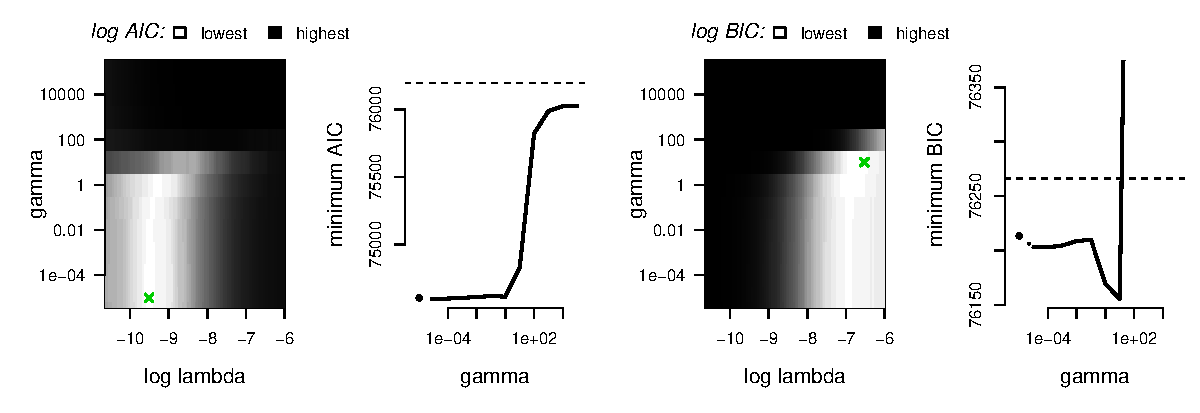
\includegraphics[width=5in]{nhl_ic}
\caption{ \label{nhlic} Hockey example AICc and BIC surfaces, rising from white to black on log scale.
}
\end{center}
% \end{figure}
% \begin{figure}[htb]
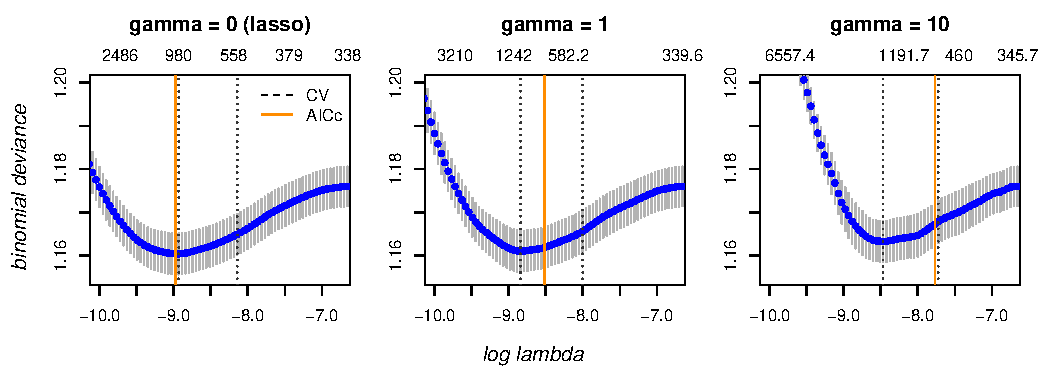
\includegraphics[width=6.3in]{nhl_cv}
\caption{\label{nhlcv} Hockey example 10-fold CV: mean OOS deviance $\pm 1$se, with minimum-error and 1SE selection rules marked with black dotted lines, and solid orange line showing AICc selection. }
\end{figure}


\begin{table}[tb]\footnotesize\setstretch{1}
\makebox[\linewidth]{
\begin{tabular}{l|lcc|lcc|lcc|}
\multicolumn{1}{c}{} & \multicolumn{3}{l}{\normalsize \it ~~~lasso} & \multicolumn{3}{l}{\normalsize \it ~~~$\gamma=1$} &  \multicolumn{3}{l}{\normalsize \it ~~~$\gamma=10$}\\
%\multicolumn{1}{c}{} & \multicolumn{3}{r|}{} & \multicolumn{3}{r|}{} &  \multicolumn{3}{r|}{}\\
\multicolumn{1}{c}{}  &     &    PPM & PM &    &   PPM & PM        &   & PPM & PM \\
\cline{3-4}\cline{6-7}\cline{9-10}
1 & Ondrej Palat & 33.8 & 38 & Sidney Crosby & 29.2 & 52 & Sidney Crosby & 32.6 & 52 \\
2 & Sidney Crosby & 31.2 & 52 & Ondrej Palat & 29 & 38 & Jonathan Toews & 22.8 & 35 \\
3 & Henrik Lundqvist & 25.8 & 9 & Jonathan Toews & 21.4 & 35 & Joe Thornton & 22 & 34 \\
4 & Jonathan Toews & 24 & 35 & Joe Thornton & 21 & 34 & Anze Kopitar & 22 & 39 \\
5 & Andrei Markov & 23.1 & 34 & Andrei Markov & 20.9 & 34 & Andrei Markov & 20.7 & 34 \\
6 & Joe Thornton & 21.4 & 34 & Henrik Lundqvist & 19.8 & 9 & Alex Ovechkin & 18.1 & 16 \\
7 & Anze Kopitar & 20.6 & 39 & Anze Kopitar & 19.5 & 39 & Pavel Datsyuk & 16.6 & 13 \\
8 & Tyler Toffoli & 18.9 & 31 & Pavel Datsyuk & 16.1 & 13 & Ryan Getzlaf & 15.8 & 16 \\
9 & Pavel Datsyuk & 17.7 & 13 & Logan Couture & 15.9 & 29 & Henrik Sedin & 15.2 & 7 \\
10 & Ryan Nugent-hopkins & 17.4 & 18 & Alex Ovechkin & 15.8 & 16 & Marian Hossa & 14.9 & 21 \\
11 & Gabriel Landeskog & 16.6 & 36 & Marian Hossa & 14.4 & 21 & Alexander Semin & 14.7 & -1 \\
12 & Logan Couture & 16.5 & 29 & Alexander Semin & 14.2 & -1 & Jaromir Jagr & 14.5 & 28 \\
13 & Alex Ovechkin & 15.8 & 16 & Matt Moulson & 13.9 & 22 & Logan Couture & 14.2 & 29 \\
14 & Marian Hossa & 15.4 & 21 & Tyler Toffoli & 13.3 & 31 & Matt Moulson & 13.7 & 22 \\
15 & Alexander Semin & 14.8 & -1 & David Perron & 12.7 & 2 & Mikko Koivu & 13 & 12 \\
16 & Zach Parise & 14.7 & 21 & Mikko Koivu & 12.5 & 12 & Joe Pavelski & 12.6 & 33 \\
17 & Frans Nielsen & 13.5 & 8 & Frans Nielsen & 12.3 & 8 & Steven Stamkos & 12.6 & 24 \\
18 & Mikko Koivu & 13.4 & 12 & Ryan Getzlaf & 12.1 & 16 & Frans Nielsen & 12.5 & 8 \\
19 & Matt Moulson & 13.4 & 22 & Ryan Nugent-hopkins & 11.9 & 18 & Marian Gaborik & 12.3 & 29 \\
20 & David Perron & 13.1 & 2 & Jaromir Jagr & 11.8 & 28 & Zach Parise & 12.2 & 21 \\
\multicolumn{1}{c}{} & \multicolumn{3}{r|}{} & \multicolumn{3}{r|}{} &  \multicolumn{3}{r|}{}\\
 \multicolumn{1}{c}{} & \multicolumn{3}{r|}{\it 305 nonzero effects} & \multicolumn{3}{r|}{\it 204 nonzero effects} &  \multicolumn{3}{r|}{\it 64 nonzero effects}
\end{tabular}}
\caption{\label{nhleffects} Top 20 AICc selected player `partial plus-minus' (PPM) values for the 2013-2014 season, under $\gamma = 0,1,10$.  The number of nonzero player effects for each $\gamma$ are noted along the bottom.}
\end{table}

The motivating application for this example was to devise a better versions of
hockey's `plus-minus' (PM) statistic: number of goals {\it for} minus {\it
against} each player's team while he is on the ice. To convert from player
effects $\beta_{0j} + \beta_{sj}$ to the scale of `plus/minus', we first state
that in absence of any other relevant information about each goal (not team,
home/away, etc), the probability a goal was scored by his team given player
$j$ is on ice becomes $p_j = e^{\beta_j}/(1+e^{\beta_j})$ and our `partial
plus/minus' (PPM) is \[ \mr{ppm}_j = N_j(p_j - (1-p_j)) = N_j(2p_j-1) \] where
$N_j$ is the  number of goals for which he was on-ice.  This measures 
quality and quantity of contribution, controlling for
confounding information, and lives on the same scale as PM.

Table \ref{nhleffects} contains the estimated PPM values for the 2013-2014
season under various $\gamma$ levels, using AICc selection.  We see that, even
if changing concavity ($\gamma$) has little effect on minimum CV errors,
larger $\gamma$  yield more sparse models and different conclusions about
player contribution. At the $\gamma=0$ lasso, there are 305 nonzero player
effects (individuals measurably different from their team's average ability)
and the list includes young players who have had very strong starts to their
careers.  For example, Ondrej Palat and Tyler Toffoli both played their first
full seasons in the NHL in 2013-2014.  As $\gamma$ increases to 1, these young
guys  drop in rank while more proven stars (e.g., Sidney Crosby and Jonathan
Toews) move up the list.  Finally, at $\gamma=10$ only big-name stars remain
amongst the 64 nonzero player effects.

\section{Discussion}
\label{discussion}


Concave penalized estimation in Big data, where exact solvers are too
computationally expensive, reduces largely to weighted-$L_1$ penalization.
This review has covered a number of topics that we think relevant for such
schemes.  Apart from the simulation study, we have not provided extensive
comparison of the many available weighting mechanisms. However, we feel that
path adaptation is an intuitively reasonable source of weights. In any case,
POSE has the advantage that using a regularization path to supply penalty
weights is computationally efficient. To scale for truly Big data, $L_1$
weights need be constructed at practically no cost on top of a standard lasso
run. Beyond {\tt gamlr} and marginal regression adaptive lasso, we have found
no other software for sparse diminishing bias estimation where this standard
is met.



\setstretch{1}
\bibliographystyle{chicago}
\bibliography{gamlr}

\setstretch{1.4}
\appendix
\vskip 1cm
\noindent{\bf\Large Appendices}

\section{Gradient, curvature, and path starts}
\label{models}

The negative log likelihood objective in Gaussian regression is $
l(\alpha,\bs{\beta}) = 0.5\sum_i (y_i -\eta_i)^2 $ with gradient
$g_j(\bs{\beta}) = \partial l/\partial \beta_j = -\sum_i x_{ij}(y_i -
\eta_i)$, and coordinate curvature $h_j(\bs{\beta}) = \partial^2 l/\partial
\beta_j^2 = \sum_i x_{ij}^2$. In logistic regression, set $y_i = 1$ for
`success' and $y_i = 0$ for `failure' and write $q_i = (1 +
\exp[-\eta_i])^{-1}$ as the probability of success.  Then
$l(\alpha,\bs{\beta}) = \sum_i -y_i\eta_i + \log(1 +
  \exp[\eta_i])$,
$
g_j(\bs{\beta}) = \partial l/\partial \beta_j = -\sum_i
x_{ij}(y_i - q_i)$, and
$h_j(\bs{\beta}) = \partial^2 l/\partial \beta_j^2 = \sum_i
x_{ij}^2q_i(1-q_i)
$.
In each case, it is implied that $\hat\alpha$ has been set
to minimize $l(\alpha,\bs{\hat\beta})$. 

For $L_1$ costs $c_j(|\beta_j|) = |\beta_j|$, the infimum $\lambda$ such
that $\bs{\hat\beta} = \bm{0}$ is  available analytically as
$\lambda^1 =
n^{-1}\max\{|g_j(\bm{0})|,~j=1\ldots p\}$, the maximum mean
absolute gradient for the null model with $\bs{\beta} = \bm{0}$.  This formula
is used to obtain our starting values for the path algorithms.

\section{Sign Recovery}
\label{extraproof}


\begin{lemma}\label{signrecov}
Under the setting of Theorem \ref{sparseapprox}, with $\hat S = \{j:\hat\beta_j \neq 0\}$, if $\omega_{S^c}^{\mr{min}}\lambda > \sqrt{2\nu}$ then
\begin{equation}
|\bs{x}_j'\bm{X}_S(\bm{X}_S'\bm{X}_S)^{-1}\bs{\omega}_S| \leq 1 - \frac{\sqrt{2\nu}}{\lambda\omega_j}~~\forall~j ~\in~S^c \Rightarrow \hat{S} \cap S^c = \varnothing.
\end{equation}
 If in addition
$\left|(\bm{X}_S'\bm{X}_S)^{-1}\bm{X}_S'\bm{y}\right|_\infty > n\lambda\left|(\bm{X}_S'\bm{X}_S)^{-1}\bs{\omega}_S\right|_\infty$, then 
$\mr{sgn}(\bs{\hat\beta}) = \mr{sgn}(\bs{\beta}^\nu)$.
\end{lemma}
\begin{proof} We adapt results of \cite{wainwright_sharp_2009}.
From the Karush-Kuhn-Tucker (KKT) conditions at weighted-$L_1$ minimization convergence, 
$\bm{x}_j'\bm{X}(\bs{\hat\beta}_S-\bs{\beta}^\nu) + \bm{X}'\bm{e}^S = -n\lambda\zeta_j$ where $|\zeta_j| = \omega_j$ for $j\in\hat S$ and $|\zeta_j| \leq \omega_j$ for $j\in\hat S^c$.
Thus we we have no false positives if and only if
\begin{equation}
\bm{X}_S'\bm{X}_S(\bs{\hat\beta}_S-\bs{\beta}^\nu_S) + \bm{X}_S'\bm{e}^S =-n\lambda\bs{\zeta}_S ~~\Rightarrow~~ \bs{\hat\beta}_S-\bs{\beta}^\nu_S = -n\lambda(\bm{X}_S'\bm{X}_S)^{-1}\bs{\zeta}_S.
\end{equation}
And all of the spurious regressors in $S^c$ will have $\hat \beta_j = 0$
if and only if
\begin{equation}
\bs{x}_j'\bm{X}_S(\bs{\hat\beta}_S-\bs{\beta}^\nu_S) - \bs{x}_j'\bm{e}^S 
\leq n\lambda\zeta_j ~~\Leftarrow~~
1 - \frac{|x_j'\bm{e}^S|}{n} \geq 1 - \frac{\sqrt{2\nu}}{\lambda\omega_j} \geq |\bs{x}_j'\bm{X}_S(\bm{X}_S'\bm{X}_S)^{-1}\bs{\omega}_S|.
\end{equation}
Finally, for sign recovery on $j\in S$ we need 
$
|\beta_j^\nu| - |\beta^\nu_j - \hat\beta_j| > 0 ~~\forall~j~\in~S
$,
and our stated condition follows from  $\bs{\beta^\nu}_S =
(\bm{X}_S'\bm{X}_S)^{-1}\bm{X}_S'\bm{y}$ and $ \bs{\beta^\nu}_S-
\bs{\hat\beta}_S = n\lambda (\bm{X}_S'\bm{X}_S)^{-1}\bs{\zeta}_S$.
\end{proof}

\section{Derivation of AIC and AICc}
\label{aicder}

Consider a Gaussian regression model where $\bs{\eta}_\bm{y}$ is an estimate
for $\bs{\eta} = \ds{E}\bm{y}$ using $df$ degrees of freedom, and set $\phi_\bm{y} =
\sigma^2_{\bm{y}} = \sum_i (y_i - \eta_{\bm{y}i})^2/n$. We'll derive
\begin{equation}\label{aiccapprox}
df\frac{n}{n-df-1}  \approx \ds{E}_{\bm{y}|g}\left[\log f(\bm{y}; \bs{\eta}_{\bm{y}},\phi_{\bm{y}}) - \ds{E}_{\bm{\tilde y}|g} \log f(\bm{\tilde y}; \bs{\eta}_{\bm{y}},\phi_{\bm{y}})
\right],
\end{equation}
such that AICc's complexity penalty is the expected bias that results from taking the fitted log likelihood as an estimate for (\ref{dualexpect}).  First, by cancellation the inner term of (\ref{aiccapprox}) simplifies as 
\begin{equation}
\log f(\bm{y}; \bs{\eta}_{\bm{y}},\phi_{\bm{y}}) - \ds{E}_{\bm{\tilde y}|g} \log f(\bm{\tilde y}; \bs{\eta}_{\bm{y}},\phi_{\bm{y}}) = 
\frac{\ds{E}_{\bm{\tilde y}|g} \sum_i (\tilde y_i - \eta_{\bm{y}i})^2}{2 \sigma^2_{\bm{y}}} - \frac{n}{2}.
\end{equation}
Now, assume that the {\it true} model is linear and that the data were generated
from $\bm{y}\sim g(\bs{\eta}, \sigma^2\bm{I})$.  The \cite{mallows_comments_1973} $C_p$ formula holds that 
$n\sigma^2_{\bm{y}} + 2 \sigma^2 df$ is an unbiased estimator for  expected 
sum of square errors $\ds{E}_{\bm{\tilde y}|g} \sum_i (\tilde y_i - \eta_{\bm{y}i})^2/n$, such that
\begin{equation}
\frac{\ds{E}_{\bm{\tilde y}|g} \sum_i (\tilde y_i - \eta_{\bm{y}i})^2}{2 \sigma^2_{\bm{y}}} - \frac{n}{2} 
 ~\approx~ \frac{n\sigma^2_{\bm{y}} + 2 \sigma^2 df}{2 \sigma^2_{\bm{y}}} - \frac{n}{2}
 ~=~  df\frac{\sigma^2 }{\sigma^2_{\bm{y}}}.
\end{equation}
At this point, we see that the standard AIC approximation results from equating $\sigma^2 \approx \ds{E}_{\bm{y}|g}\sigma^2_{\bm{y}}$, so that $df\ds{E}_{\bm{y}|g}[\sigma^2/\sigma^2_{\bm{y}}] \approx df$.  This will underpenalize complexity whenever residual variance $\sigma^2_{\bm{y}}$ tends to be smaller than the true variance $\sigma^2$  -- that is, whenever the model is overfit.  In contrast, AICc applies the chi-squared goodness of fit result $
{n\sigma^2_{\bm{y}}/\sigma^2} \sim \chi^2_{n-df-1}
$
to obtain 
\begin{equation}
\ds{E}_{\bm{y}|g}\left[\frac{\sigma^2 }{\sigma^2_{\bm{y}}}df\right]= 
n\ds{E}_{\bm{y}|g}\left[\frac{1}{n\sigma^2_{\bm{y}}/\sigma^2}\right]df = 
\frac{n}{n-df-1}df.
\end{equation}
Multiplying by $-2$ and subtracting from $-2\log f(\bm{y}; \bs{\eta}_{\bm{y}},\sigma_{\bm{y}})$ yields the AICc.


\section{Implementation via coordinate descent}
\label{implement}

We use Coordinate descent \citep[CD; e.g.,][]{luenberger_linear_2008} to minimize
(\ref{l1pen}) at each step along the path. CD is a local optimization
algorithm that cycles through minimization of the conditional objective for
individual parameters when the remaining parameters are fixed. Algorithms of this type have have become popular in
$L_1$ penalized estimation since the work by \citet{friedman_pathwise_2007} and
\citet{wu_coordinate_2008}.

Our CD routine, outlined in Algorithm \ref{bmove}, is a solver for penalized
weighted-least squares problems as defined in equation (\ref{newton}) below.
This applies directly in Gaussian regression, and for non-Gaussian models  we
follow \citet{friedman_regularization_2010} and apply CD inside an outer loop
of iteratively re-weighted-least-squares \citep[IRLS;
e.g.,][]{green_iteratively_1984}. Given current parameter values
$\bs{\hat\beta}$, the Newton-Raphson update for maximum likelihood estimation
is $\bs{\beta} = \bs{\hat\beta} - \bm{H}^{-1}\bm{g}$, where $\bm{H}$ is the
information matrix with elements $h_{jk} = \partial^2 l/\partial
\beta_j\partial \beta_k |_{\bs{\hat\beta}}$ and $\bm{g}$ is coefficient
gradient (see Appendix \ref{models}). For exponential family linear models we
can write $\bm{H} = \bm{X}'\bm{V}\bm{X}$ and $\bm{g} = \bm{X}'\bm{V}(\bm{z} -
\bs{\hat\eta})$, where $\bm{V} = \mr{diag}(\bm{v})$, $\bm{v} = [v_1\ldots
v_n]$ are `weights', $\bm{z} = [z_1\ldots z_n]$ are transformed `response',
and $\hat\eta_i = \hat\alpha + \bm{x}_i\bs{\hat\beta}$.  In Gaussian
regression,  $v_i = 1$, $z_i=\hat\eta_i - y_i$, and the update is an exact
solution. For binomial regression, $v_i = q_i(1-q_i)$ and $z_i = \hat\eta_i -
(y_i-q_i)/v_i$, where $q_i = (1 + \exp[-\hat\eta_i])^{-1}$ is the  estimated
probability of success.

This yields $\bs{\beta} = (\bm{X}'\bm{V}\bm{X})^{-1}\bm{X}'\bm{V}\bm{z}$, such
that the Newton update solves a weighted-least-squares problem.   Adding $L_1$
costs,  the minimization objective from (\ref{l1pen}) becomes
\begin{equation} \label{newton}  \argmin_{\alpha,\beta_1 \ldots \beta_p \in
\ds{R}} \sum_i \frac{v_i}{2}(\alpha + \bm{x}_i'\bs{\beta} - z_i)^2  + n\sum_j \omega_j
\lambda |\beta_j|. \end{equation} Our solver iterates between CD on
(\ref{newton}) and,  for non-Gaussian models, updates to $\bm{v}$ and
$\bm{z}$. Each $t^{th}$ segment IRLS routine initializes $[\hat \alpha,
\bs{\hat \beta}]$ at solutions for $\lambda^{t-1}$, or at $[\hat \alpha,
\bm{0}]$ for $t=1$.  In the {\tt gamlr} implementation, a full pass update of
all parameters is done only at the first CD iteration; otherwise coordinates
with currently inactive (zero) $\hat\beta_j$ are not updated. Once the descent
converges for this {\it active set}, IRLS $\bm{v}$ and $\bm{z}$ are updated
and we begin a new CD loop with a full pass update.  The routine stops when
maximum squared change in $\beta_j$ scaled by its information over one of
these full pass updates is less than some tolerance threshold, ${\tt thresh}$.
The default in {\tt gamlr} uses a relative tolerance of $10^{-7}$ times null
model deviance.  

\vspace{.25cm}
\begin{algorithm}[ht]
\vspace{.25cm}
\caption{Coordinate descent\label{bmove}}

\vskip .15cm
\hskip .5cm Set ${\tt vh_j} = \sum_i v_i(x_{ij} - \bar x_j)^2$ 
and ${\tt vx_j} = \sum_i v_ix_{ij}$ for $j=1\ldots p$.

\vskip .15cm
\hskip .5cm while $\displaystyle \max_{j = 1\ldots p} {\tt vh_j}\Delta_j^2 > {\tt thresh}$:

\vskip .15cm
\hskip 1.5cm for {j=1\ldots p}:


\vskip .15cm
\hskip 2.5cm set ${\tt vg_j} = -\sum_i x_{ij}v_i(z_i-\hat\eta_i)$ and ${\tt ghb} = {\tt vg_j} - {\tt vh_j}\hat\beta_j$


\vskip .25cm
\hskip 2.5cm if $|{\tt ghb}| < n\lambda^t\omega^t_j$:~ $\Delta_j = -\hat\beta_j$

\vskip .1cm
\hskip 2.5cm else:~ $\Delta_j = -({\tt vg_j} - \mr{sign}({\tt ghb}) n\lambda^t\omega^t_j)/{\tt vh_j}$.

\vskip .25cm
\hskip 2.5cm  update $\hat\beta_j \stackrel{+}{=} \Delta_j$,
$\hat\alpha \stackrel{+}{=} -{\tt vx_j}\Delta_j$, 
and $\bs{\hat\eta} = \hat\alpha + \bm{X}'\bs{\hat\beta}$.

\vskip .25cm

\end{algorithm}


\subsection{Descent convergence}

 Despite the non-differentiability of $|\beta_j|$ at zero,
\citet{tseng_convergence_2001} establishes local convergence for CD on
(\ref{newton}) as a consequence of penalty separability: the
non-differentiable part of our objective is a sum of functions on only a
single coordinate.  Thus CD solves each weighted-least squares problem, and
the full algorithm converges if IRLS does.  For non-Gaussian models,
convergence of such nested $L_1$-penalized IRLS algorithms is shown
in \cite{lee_proximal_2014}.

\subsection{Quasi-Newton acceleration}
\label{qn}

Under high collinearity and large $\gamma$, one may wish to accelerate convergence via a quasi-Newton step
\citep[e.g.,][]{lange_numerical_2010}. Acceleration is applied to $\bs{\theta}
= [\alpha,\bs{\beta}]$, and a move is accepted only if it leads to a decrease
in the objective. Suppose that $\bs{\hat\theta}^{(0)}$,
$\bs{\hat\theta}^{(-1)}$, and $\bs{\hat\theta}^{(-2)}$ are the current,
previous, and previous-to-previous parameter estimates.  Write
$M(\bs{\hat\theta}^{(t)})$ as the implied CD update map $\bs{\hat\theta}^{(t)}
\rightarrow \bs{\hat\theta}^{(t+1)}$, such that the algorithm converges at
$\bs{\hat\theta} - M(\bs{\hat\theta}) = \bm{0}$.  With $\bm{u} =
\bs{\hat\theta}^{(-1)} - \bs{\hat\theta}^{(-2)}$ and $\bm{v} =
\bs{\hat\theta}^{(0)} - \bs{\hat\theta}^{(-1)}$, a secant approximation to the
gradient of $M$ is $\partial M/\partial \hat\theta_l \approx
\mr{v}_l/\mr{u}_l$.  An approximate Newton-Raphson step to solve for the root
of $\bs{\hat\theta} - M(\bs{\hat\theta}) $  updates each coordinate $\hat
\theta_l \gets \hat\theta_l^{(-1)} - (\hat\theta_l^{(-1)} -
\hat\theta_l^{(0)})/(1-\mr{v}_l/\mr{u}_l)$ which can be re-written as
$\hat\theta_l = (1-\mr{w}_l)\hat\theta_l^{(-1)} + \mr{w}_l\hat\theta_l^{(0)} $
where $\mr{w}_l = \mr{u}_l/(\mr{u}_l - \mr{v}_l)$.



\end{document}

